%Version 3.1 December 2024
% See section 11 of the User Manual for version history
%
%%%%%%%%%%%%%%%%%%%%%%%%%%%%%%%%%%%%%%%%%%%%%%%%%%%%%%%%%%%%%%%%%%%%%%
%%                                                                 %%
%% Please do not use \input{...} to include other tex files.       %%
%% Submit your LaTeX manuscript as one .tex document.              %%
%%                                                                 %%
%% All additional figures and files should be attached             %%
%% separately and not embedded in the \TeX\ document itself.       %%
%%                                                                 %%
%%%%%%%%%%%%%%%%%%%%%%%%%%%%%%%%%%%%%%%%%%%%%%%%%%%%%%%%%%%%%%%%%%%%%

%%\documentclass[referee,sn-basic]{sn-jnl}% referee option is meant for double line spacing

%%=======================================================%%
%% to print line numbers in the margin use lineno option %%
%%=======================================================%%

%%\documentclass[lineno,pdflatex,sn-basic]{sn-jnl}% Basic Springer Nature Reference Style/Chemistry Reference Style

%%=========================================================================================%%
%% the documentclass is set to pdflatex as default. You can delete it if not appropriate.  %%
%%=========================================================================================%%

%%\documentclass[sn-basic]{sn-jnl}% Basic Springer Nature Reference Style/Chemistry Reference Style

%%Note: the following reference styles support Namedate and Numbered referencing. By default the style follows the most common style. To switch between the options you can add or remove “Numbered” in the optional parenthesis. 
%%The option is available for: sn-basic.bst, sn-chicago.bst%  
 
%%\documentclass[pdflatex,sn-nature]{sn-jnl}% Style for submissions to Nature Portfolio journals
%%\documentclass[pdflatex,sn-basic]{sn-jnl}% Basic Springer Nature Reference Style/Chemistry Reference Style
\documentclass[lineno,pdflatex,sn-nature]{sn-jnl}% Math and Physical Sciences Numbered Reference Style
%%\documentclass[pdflatex,sn-mathphys-ay]{sn-jnl}% Math and Physical Sciences Author Year Reference Style
%%\documentclass[pdflatex,sn-aps]{sn-jnl}% American Physical Society (APS) Reference Style
%%\documentclass[pdflatex,sn-vancouver-num]{sn-jnl}% Vancouver Numbered Reference Style
%%\documentclass[pdflatex,sn-vancouver-ay]{sn-jnl}% Vancouver Author Year Reference Style
%%\documentclass[pdflatex,sn-apa]{sn-jnl}% APA Reference Style
%%\documentclass[pdflatex,sn-chicago]{sn-jnl}% Chicago-based Humanities Reference Style

%%%% Standard Packages
%%<additional latex packages if required can be included here>

\usepackage{graphicx}%
\usepackage{multirow}%
\usepackage{amsmath,amssymb,amsfonts}%
\usepackage{amsthm}%
\usepackage{mathrsfs}%
\usepackage[title]{appendix}%
\usepackage{xcolor}%
\usepackage{textcomp}%
\usepackage{manyfoot}%
\usepackage{booktabs}%
\usepackage{algorithm}%
\usepackage{algorithmicx}%
\usepackage{algpseudocode}%
\usepackage{listings}%


\raggedbottom
%%\unnumbered% uncomment this for unnumbered level heads

\begin{document}

\title[Article Title]{Range shifts offer little thermal or demographic relief}

\author*[1]{\fnm{Federico} \sur{Maioli}}\email{fedma@aqua.dtu.dk} 
\author[1]{\fnm{Daniël} \spfx{van}\sur{Denderen}}\email{pdvd@aqua.dtu.dk} %surnameprefix? 
\author[2]{\fnm{Max} \sur{Lindmark}}\email{max.lindmark@slu.se}  
\author[1]{\fnm{Marcel} \sur{Montanyès}}\email{mamont@aqua.dtu.dk}  
\author[3]{\fnm{Eric\,J.} \sur{Ward}}\email{eric.ward@noaa.gov}  
\author[4]{\fnm{Sean\,C.} \sur{Anderson}}\email{sean.anderson@dfo-mpo.gc.ca}  
\author[1]{\fnm{Martin} \sur{Lindegren}}\email{mli@aqua.dtu.dk} 

\affil*[1]{\orgdiv{National Institute of Aquatic Resources}, \orgname{Technical University of Denmark (DTU)}, \orgaddress{\street{Henrik Dams Allé 202}, \city{Kongens Lyngby}, \postcode{2800}, \country{Denmark}}}  

\affil[2]{\orgdiv{Department of Aquatic Resources}, \orgname{Swedish University of Agricultural Sciences (SLU)}, \orgaddress{\street{Turistgatan 5}, \city{Lysekil}, \postcode{45330}, \country{Sweden}}}  

\affil[3]{\orgdiv{Conservation Biology Division}, \orgname{NOAA Fisheries, Northwest Fisheries Science Center}, \orgaddress{\street{2725 Montlake Blvd E}, \city{Seattle}, \postcode{WA 98112}, \country{USA}}}  

\affil[4]{\orgdiv{Pacific Biological Station}, \orgname{Fisheries and Oceans Canada}, \orgaddress{\street{3190 Hammond Bay Rd}, \city{Nanaimo}, \postcode{BC V9T 6N7}, \country{Canada}}}  

%%==================================%%
%% Sample for unstructured abstract %%
%%==================================%%
% 200 words
\abstract{}

%%================================%%
%% Sample for structured abstract %%
%%================================%%

% \abstract{\textbf{Purpose:} The abstract serves both as a general introduction to the topic and as a brief, non-technical summary of the main results and their implications. The abstract must not include subheadings (unless expressly permitted in the journal's Instructions to Authors), equations or citations. As a guide the abstract should not exceed 200 words. Most journals do not set a hard limit however authors are advised to check the author instructions for the journal they are submitting to.
% 
% \textbf{Methods:} The abstract serves both as a general introduction to the topic and as a brief, non-technical summary of the main results and their implications. The abstract must not include subheadings (unless expressly permitted in the journal's Instructions to Authors), equations or citations. As a guide the abstract should not exceed 200 words. Most journals do not set a hard limit however authors are advised to check the author instructions for the journal they are submitting to.
% 
% \textbf{Results:} The abstract serves both as a general introduction to the topic and as a brief, non-technical summary of the main results and their implications. The abstract must not include subheadings (unless expressly permitted in the journal's Instructions to Authors), equations or citations. As a guide the abstract should not exceed 200 words. Most journals do not set a hard limit however authors are advised to check the author instructions for the journal they are submitting to.
% 
% \textbf{Conclusion:} The abstract serves both as a general introduction to the topic and as a brief, non-technical summary of the main results and their implications. The abstract must not include subheadings (unless expressly permitted in the journal's Instructions to Authors), equations or citations. As a guide the abstract should not exceed 200 words. Most journals do not set a hard limit however authors are advised to check the author instructions for the journal they are submitting to.}

\keywords{Climate tracking, Range shifts, Thermal niche, Winner-loser}

\maketitle

\section{Introduction}\label{Introduction}
The world's ocean are warming rapidly, driving a major reorganization of marine biodiversity \citep{ipcc_ocean_2019}. As temperature rise, species are expected to track their thermal niches ---the temperature ranges suitable for their survival and reproduction \citep{grinnell_niche-relationships_1917}---by shifting their geographic distributions. Widespread poleward and deepward movements have been documented across taxa and regions, suggesting one of the most pervasive and coherent biological responses to climate change \citep{parmesan_globally_2003, parmesan_ecological_2006, poloczanska_global_2013, poloczanska_responses_2016}. Yet, many populations deviate from these expectations, remaining stationary or even shifting in unexpected directions \citep{fuchs_wrong-way_2020, lawlor_mechanisms_2024}. Regardless of direction, such redistributions are reshaping marine ecosystems, altering food webs, challenging resource management, and redefining conservation priorities worldwide \citep{pinsky_preparing_2018, palacios-abrantes_climate_2025, pecl_biodiversity_2017}.

Despite extensive documentation of range shifts, most studies track shifts along a single environmental gradient—typically latitude, or less often, depth \citep{nye_changing_2009, dulvy_climate_2008, pinsky_marine_2013}. Focusing on one gradient at a time oversimplifies species’ responses to ocean warming and may help explain why predictions of range shifts—both in magnitude and direction—often fall short \citep{lawlor_mechanisms_2024, fredston_reimagining_2025}. As a result, our ability to anticipate future changes in species distributions and to manage their consequences remains limited. In reality, marine species are unlikely to respond to warming along one gradient alone. They may shift horizontally, move vertically into cooler waters, remain in place while tolerating greater thermal exposure, or combine these strategies \citep{nye_changing_2009}. Thus, considering shifts along multiple gradients and their potential interactions offers a more realistic representation of climate-driven redistribution of marine fishes.

%% from here
%Here, we develop a multidimensional framework to quantify spatial redistribution of marine species, capturing changes across both horizontal and vertical axes. By integrating these components, we aim to identify consistent patterns of thermal tracking, evaluate departures from expectation, and provide a more comprehensive view of how marine biodiversity is reorganizing in response to ocean warming.
To that end, we here develop and apply a multidimensional framework that considers three complementary dimensions of climate response: (i) horizontal range shifts, captured through changes in range centroids; (ii) vertical redistributions, reflected in realized depth niches; and
(iii) changes in realized thermal niches. This framework allows us to evaluate not only the direction and magnitude of spatial movements, but also whether such movements effectively track shifting thermal environments. If populations perfectly follow changing isotherms, their realized thermal niches should remain stable over time despite environmental warming. Conversely, systematic trends in thermal niche temperature would signal incomplete tracking and increasing thermal exposure.
Finally, to understand whether redistribution effectively buffers species from climate impacts, we link spatial and thermal adjustments to long-term abundance trends, testing whether movement strategies confer demographic resilience under ocean warming.
However, movement alone does not ensure persistence—species may shift yet continue to face warming, or remain stationary while maintaining stable populations. To determine whether redistribution effectively buffers species from climate impacts, we link spatial and thermal adjustments to long-term abundance trends, testing whether movement strategies confer demographic resilience under ocean warming.

Our study draws on a comprehensive set of standardized scientific bottom-trawl surveys, including more than 200 well sampled demersal (bottom-living) fish populations across 11 regions of the North Atlantic and Northeast Pacific. These regions include some of the fastest-warming continental shelf seas \citep{pershing_slow_2015, song_arctic_2023}, span broad latitudinal and climatic gradients, and contain some of the most comprehensive long-term records of marine biodiversity change \citep{maureaud_are_2021, maureaud_fishglob_data_2024}. Together, these contrasts in climate exposure and exceptional data coverage make these regions a natural laboratory for understanding how marine species respond to ocean warming.

We use spatiotemporal and Bayesian mixed-effects models to quantify long-term trends in species’ range centroids, depth distributions, and thermal niches. By examining patterns both within and across regions, we identify common strategies of climate response and assess which are most effective at reducing thermal exposure. Finally, we link these strategies to long-term abundance trends to evaluate whether species that better track changing conditions maintain more stable populations.
%Finally, we test whether these strategies are associated with changes in population abundance, potentially distinguishing species that are adapting to warming conditions from those in decline.



%These regions include some of the fastest-warming continental shelf seas \citep{pershing_slow_2015, song_arctic_2023}, span broad latitudinal and climatic gradients, and provide some of the world's most comprehensive long-term records of marine biodiversity change \citep{maureaud_are_2021, maureaud_fishglob_data_2024}. 



%Continental shelfs sustain exceptional biodiversity and productivity, support some of the world’s largest fisheries, and contribute roughly X\% of the global marine catch \citep{watson_database_2017}. Shelf systems also experience warming at rates exceeding the global ocean average , exposing resident species to accelerated thermal stress. Thus, continental shelves support high biodiversity and productivity while facing disproportionate exposure to climate-driven warming.

 
 


%or We hypothesize that if populations perfectly track shifting temperatures, their realized thermal niches should remain stable through time despite environmental warming.

%By linking these spatial and thermal responses to long-term abundance trends, we test whether movement can buffer populations and sustain demographic resilience under climate change.

%These regions include some of the fastest-warming continental shelf seas \citep{pershing_slow_2015, song_arctic_2023}, spanning broad latitudinal and climatic gradients and containing some of the most comprehensive long-term records of marine biodiversity change \citep{maureaud_are_2021, maureaud_fishglob_data_2024}. Together, these contrasts in climate exposure and exceptional data coverage make continental shelves a natural laboratory for understanding how marine species respond to ocean warming.

%are effective in buffering fromrising temperatures

%%%% Second part

%Embracing this multidimensional perspective marks an essential step toward improving our ability to monitor, model, and manage species on the move.



%However,  Considering shifts in multiple directions and their potential interactions offers a more realistic representation of climate-driven redistribution of marine fishes. If populations perfectly track temperature, their niche should remain stable over time despite enviornmetnal warmig. In contrast, tredns in termal nich temperature would signal incomplete tracking. 


%Critically, these two missing pieces—considering multidimensional redistribution and linking shifts to demographic outcomes—are essential for understanding how populations cope with warming and whether movements effectively buffer species from thermal stress. 


%A further uncertainty is whether these redistributions actually mitigate thermal stress or translate into demographic benefits. Movement alone does not guarantee persistence under climate change—species may shift yet still experience warming, or remain stationary while maintaining stable populations. Understanding how spatial and thermal adjustments interact, and whether they confer resilience or risk, requires a multidimensional perspective that links redistribution to exposure and abundance outcomes.

% or remaining in place while tolerating or adapting to thermal change. It is also unclear wether movements or lack thereof help them persist under warming. 

 % this is also nice
%Despite the ubiquity of observed shifts, predictions of their direction and magnitude frequently fall short \citep{lawlor_mechanisms_2024, fredston_reimagining_2025}. One key reason is that most studies track redistribution along a single gradient—typically latitude, or less commonly, depth \citep{pinsky_marine_2013, dulvy_climate_2008}. This unidimensional focus overlooks how species respond simultaneously along multiple, interacting axes. In reality, marine populations can shift horizontally, redistribute vertically into cooler waters, or remain in place while tolerating increased thermal exposure \citep{nye_changing_2009}. Such multidimensional responses complicate how we interpret redistribution and may help explain persistent model mismatches between predicted and observed shifts.

%Evaluating these multidimensional responses together is essential to understand not only how species redistribute, but whether such movements effectively buffer populations from demographic decline.


%Our analysis combines these redistribution metrics with long-term trends in population abundance, providing a rare opportunity to link spatial and demographic responses to climate change. Drawing on standardized bottom-trawl surveys for more than 200 demersal fish populations across 11 continental shelf regions of the North Atlantic and Northeast Pacific—among the fastest-warming marine ecosystems globally—we use spatiotemporal and Bayesian mixed-effects models to quantify shifts in range, depth, and temperature niches. We then identify whether distinct combinations of responses form coherent redistribution strategies and evaluate whether these strategies are associated with population growth or decline, thereby testing whether movement confers demographic resilience under ocean warming.

%Species are on the move in response to rapidly warming oceans, with many expected to shift poleward or into deeper waters to track their thermal niches—the ranges of temperatures suitable for survival and reproduction \citep{grinnell_niche-relationships_1917, poloczanska_global_2013}. Yet predictions of the direction and magnitude of these shifts often fall short \citep{lawlor_mechanisms_2024, fredston_reimagining_2025}, limiting our ability to anticipate changes in species distributions and to design effective management and conservation strategies. One key reason for this shortfall is that most studies examine redistribution along a single axis, such as latitude or depth \citep{pinsky_marine_2013, dulvy_climate_2008}. In reality, marine species can respond along multiple dimensions simultaneously: . Critically, understanding both the multidimensional nature of redistribution and whether such movements confer demographic benefits is essential for assessing how species cope with ocean warming.


\section{Results}\label{Results}
\newcommand{\cogxc_median}{-1.45}
\newcommand{\cogxc_value}{-1.45 (95\% CI: -6.76--2.51)}
\newcommand{\cogyc_median}{0.63}
\newcommand{\cogyc_value}{0.63 (95\% CI: -4.27--6.51)}
\newcommand{\depthnichec_median}{0.25}
\newcommand{\depthnichec_value}{0.25 (95\% CI: -0.40--1.03)}
\newcommand{\thermalnichec_median}{0.18}
\newcommand{\thermalnichec_value}{0.18 (95\% CI: 0.07--0.30)}


\subsection{No net spatial shifts, but widespread niche warming across species and regions}

Overall, we found no consistent directional shifts across species and regions in either latitude or longitude over time, as indicated by 95\% Credible Intervals (CIs) overlapping zero. In our Bayesian regression model, the posterior mean global slope ($\beta_{\text{decade}}$) for latitudinal shift was 0.35 km decade$^{-1}$ [95\% CI: -8.04, 8.82], and for longitudinal shift was -2.73 km decade$^{-1}$ [95\% CI: -8.82, 2.88] (Fig. \ref{fig:posterior_slopes}). In contrast, we observed modest support for cross-regional trends in species deepening and strong support for thermal niche warming. The global slope for depth shift was 0.6 m decade$^{-1}$ [95\% CI: -0.53, 1.64], whereas for thermal niche shift it was 0.18 $^{\circ}$C decade$^{-1}$ [95\% CI: 0.07, 0.29] (Fig. \ref{fig:posterior_slopes}a).

\begin{figure}[h]
\centering
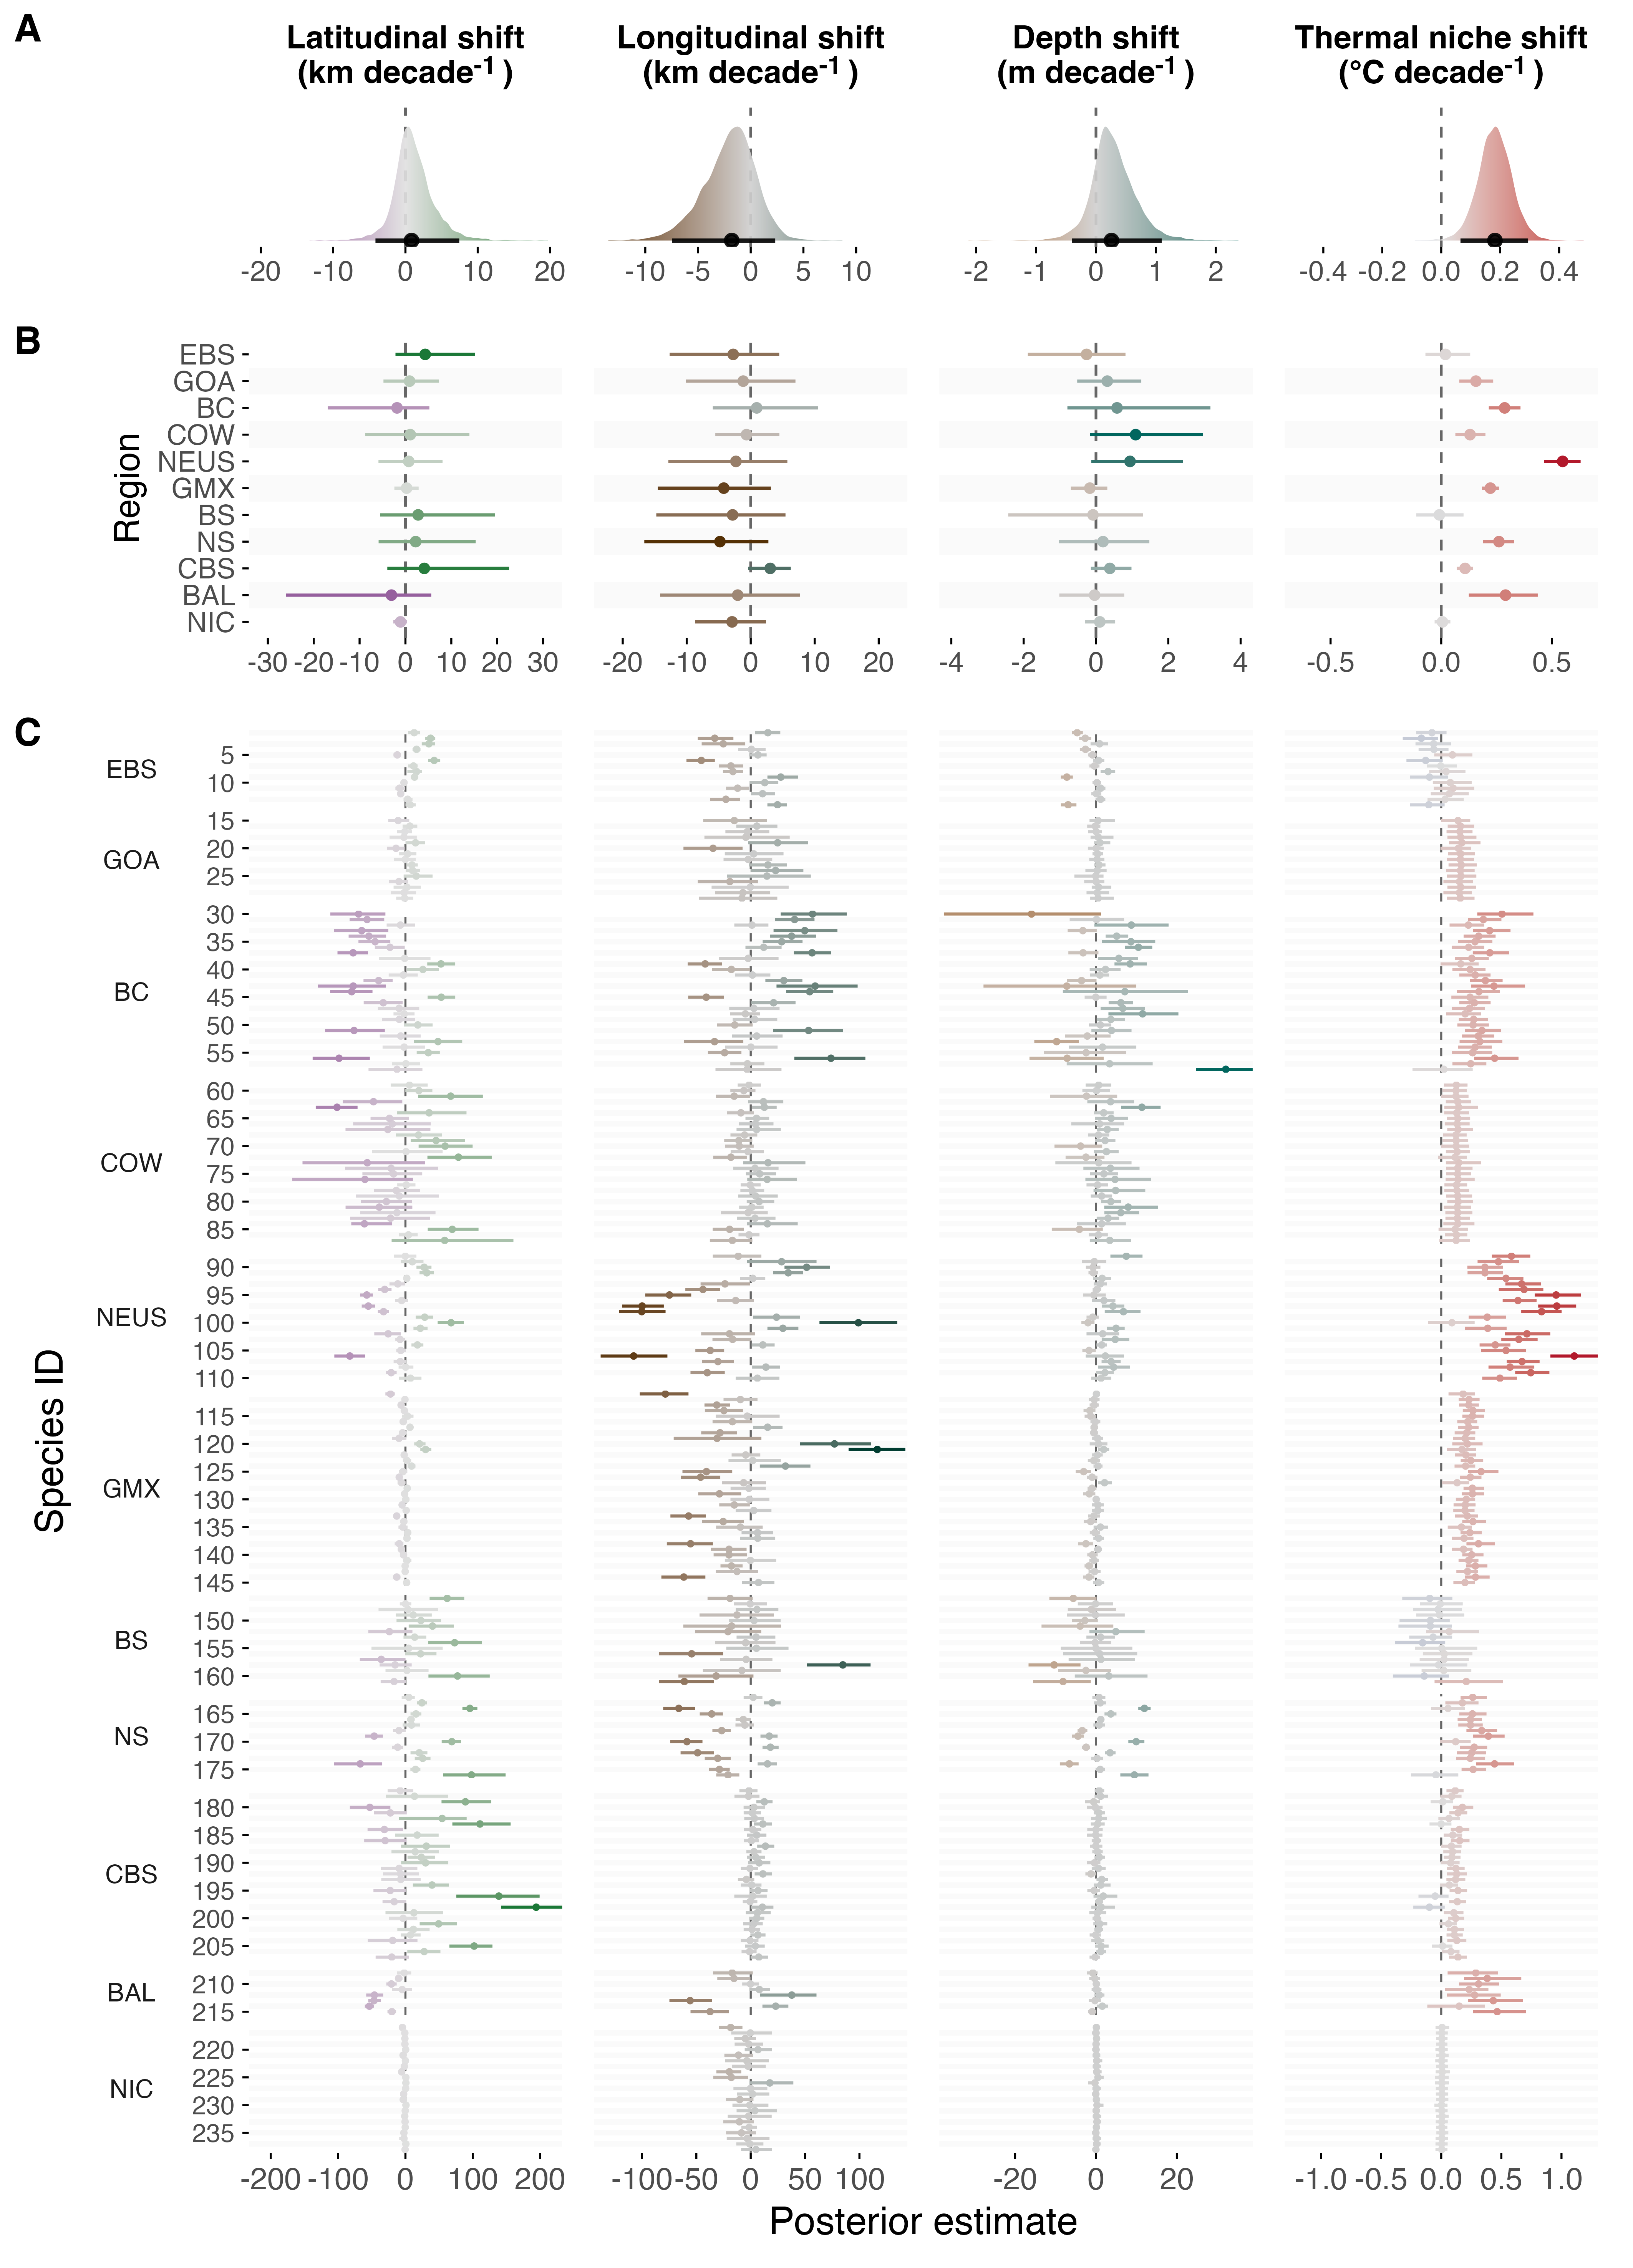
\includegraphics[width=1\textwidth]{output/figures/main/posterior_slopes.png}
\label{fig:posterior_slopes}
\caption{Trends in distributional shifts of demersal fish species over time, from left to right: latitudinal, longitudinal, depth, and thermal niche shifts. Points and horizontal lines indicate posterior medians and 95\% Bayesian credible intervals.  
(a) Global posterior slopes ($\beta_{year}$),  
(b) Region-specific trends,  
(c) Species-specific trends (rows represent species within regions; see Supplementary XX).  
Density intervals in (a-b) use a continuous gradient reflecting x-values; in (c), color represents median effect size, with more intense colors indicating larger deviations from zero.  
Marine regions: COW = California-Oregon-Washington, NEUS = Northeast U.S. and Scotian Shelf, BS = Barents Sea, NS = North Sea, BC = British Columbia, GOA = Gulf of Alaska, GMX = Gulf of Mexico, NIC = Northern Iberian Coast, EBS = Eastern Bering Sea, CBS = Celtic-Biscay Shelf, BAL = Baltic Sea.}
\end{figure}


\section{This is an example for first level head---section head}\label{sec3}

\subsection{This is an example for second level head---subsection head}\label{subsec2}

\subsubsection{This is an example for third level head---subsubsection head}\label{subsubsec2}

Sample body text. Sample body text. Sample body text. Sample body text. Sample body text. Sample body text. Sample body text. Sample body text. 

\section{Equations}\label{sec4}

Equations in \LaTeX\ can either be inline or on-a-line by itself (``display equations''). For
inline equations use the \verb+$...$+ commands. E.g.: The equation
$H\psi = E \psi$ is written via the command \verb+$H \psi = E \psi$+.

For display equations (with auto generated equation numbers)
one can use the equation or align environments:
\begin{equation}
\|\tilde{X}(k)\|^2 \leq\frac{\sum\limits_{i=1}^{p}\left\|\tilde{Y}_i(k)\right\|^2+\sum\limits_{j=1}^{q}\left\|\tilde{Z}_j(k)\right\|^2 }{p+q}.\label{eq1}
\end{equation}
where,
\begin{align}
D_\mu &=  \partial_\mu - ig \frac{\lambda^a}{2} A^a_\mu \nonumber \\
F^a_{\mu\nu} &= \partial_\mu A^a_\nu - \partial_\nu A^a_\mu + g f^{abc} A^b_\mu A^a_\nu \label{eq2}
\end{align}
Notice the use of \verb+\nonumber+ in the align environment at the end
of each line, except the last, so as not to produce equation numbers on
lines where no equation numbers are required. The \verb+\label{}+ command
should only be used at the last line of an align environment where
\verb+\nonumber+ is not used.
\begin{equation}
Y_\infty = \left( \frac{m}{\textrm{GeV}} \right)^{-3}
    \left[ 1 + \frac{3 \ln(m/\textrm{GeV})}{15}
    + \frac{\ln(c_2/5)}{15} \right]
\end{equation}
The class file also supports the use of \verb+\mathbb{}+, \verb+\mathscr{}+ and
\verb+\mathcal{}+ commands. As such \verb+\mathbb{R}+, \verb+\mathscr{R}+
and \verb+\mathcal{R}+ produces $\mathbb{R}$, $\mathscr{R}$ and $\mathcal{R}$
respectively (refer Subsubsection~\ref{subsubsec2}).

\section{Tables}\label{sec5}

Tables can be inserted via the normal table and tabular environment. To put
footnotes inside tables you should use \verb+\footnotetext[]{...}+ tag.
The footnote appears just below the table itself (refer Tables~\ref{tab1} and \ref{tab2}). 
For the corresponding footnotemark use \verb+\footnotemark[...]+

\begin{table}[h]
\caption{Caption text}\label{tab1}%
\begin{tabular}{@{}llll@{}}
\toprule
Column 1 & Column 2  & Column 3 & Column 4\\
\midrule
row 1    & data 1   & data 2  & data 3  \\
row 2    & data 4   & data 5\footnotemark[1]  & data 6  \\
row 3    & data 7   & data 8  & data 9\footnotemark[2]  \\
\botrule
\end{tabular}
\footnotetext{Source: This is an example of table footnote. This is an example of table footnote.}
\footnotetext[1]{Example for a first table footnote. This is an example of table footnote.}
\footnotetext[2]{Example for a second table footnote. This is an example of table footnote.}
\end{table}

\noindent
The input format for the above table is as follows:

%%=============================================%%
%% For presentation purpose, we have included  %%
%% \bigskip command. Please ignore this.       %%
%%=============================================%%
\bigskip
\begin{verbatim}
\begin{table}[<placement-specifier>]
\caption{<table-caption>}\label{<table-label>}%
\begin{tabular}{@{}llll@{}}
\toprule
Column 1 & Column 2 & Column 3 & Column 4\\
\midrule
row 1 & data 1 & data 2	 & data 3 \\
row 2 & data 4 & data 5\footnotemark[1] & data 6 \\
row 3 & data 7 & data 8	 & data 9\footnotemark[2]\\
\botrule
\end{tabular}
\footnotetext{Source: This is an example of table footnote. 
This is an example of table footnote.}
\footnotetext[1]{Example for a first table footnote.
This is an example of table footnote.}
\footnotetext[2]{Example for a second table footnote. 
This is an example of table footnote.}
\end{table}
\end{verbatim}
\bigskip
%%=============================================%%
%% For presentation purpose, we have included  %%
%% \bigskip command. Please ignore this.       %%
%%=============================================%%

\begin{table}[h]
\caption{Example of a lengthy table which is set to full textwidth}\label{tab2}
\begin{tabular*}{\textwidth}{@{\extracolsep\fill}lcccccc}
\toprule%
& \multicolumn{3}{@{}c@{}}{Element 1\footnotemark[1]} & \multicolumn{3}{@{}c@{}}{Element 2\footnotemark[2]} \\\cmidrule{2-4}\cmidrule{5-7}%
Project & Energy & $\sigma_{calc}$ & $\sigma_{expt}$ & Energy & $\sigma_{calc}$ & $\sigma_{expt}$ \\
\midrule
Element 3  & 990 A & 1168 & $1547\pm12$ & 780 A & 1166 & $1239\pm100$\\
Element 4  & 500 A & 961  & $922\pm10$  & 900 A & 1268 & $1092\pm40$\\
\botrule
\end{tabular*}
\footnotetext{Note: This is an example of table footnote. This is an example of table footnote this is an example of table footnote this is an example of~table footnote this is an example of table footnote.}
\footnotetext[1]{Example for a first table footnote.}
\footnotetext[2]{Example for a second table footnote.}
\end{table}

\begin{sidewaystable}
\caption{Summary of annual spatial and thermal metrics used to quantify species’ distributional and thermal responses to ocean warming}
\label{table:derived_quantities}
\centering
\renewcommand{\arraystretch}{1.5}
\begin{tabular}{@{}p{3.2cm}p{3.5cm}p{5cm}p{4.3cm}@{}}
\toprule
Name & Metric & Definition / Formula & Interpretation \\
\midrule
Range centroid (UTM northing) & Density-weighted northing &
$\bar{y} = \frac{\sum y_i D_i}{\sum D_i}$, where $y_i$ is the UTM northing of grid cell $i$, and $D_i$ is predicted density. &
Tracks north–south distributional shifts. \\
Range centroid (UTM easting) & Density-weighted easting &
$\bar{x} = \frac{\sum x_i D_i}{\sum D_i}$, where $x_i$ is the UTM easting of grid cell $i$. &
Tracks east–west distributional shifts. \\
Depth niche & Density-weighted depth &
$\bar{z} = \frac{\sum z_i D_i}{\sum D_i}$, where $z_i$ is depth in grid cell $i$. &
Captures changes in vertical habitat use. \\
Thermal niche & Density-weighted temperature &
$\bar{T} = \frac{\sum T_i D_i}{\sum D_i}$, where $T_i$ is bottom temperature in grid cell $i$. &
Reflects thermal conditions in occupied habitat. \\
\botrule
\end{tabular}
\end{sidewaystable}

In case of double column layout, tables which do not fit in single column width should be set to full text width. For this, you need to use \verb+\begin{table*}+ \verb+...+ \verb+\end{table*}+ instead of \verb+\begin{table}+ \verb+...+ \verb+\end{table}+ environment. Lengthy tables which do not fit in textwidth should be set as rotated table. For this, you need to use \verb+\begin{sidewaystable}+ \verb+...+ \verb+\end{sidewaystable}+ instead of \verb+\begin{table*}+ \verb+...+ \verb+\end{table*}+ environment. This environment puts tables rotated to single column width. For tables rotated to double column width, use \verb+\begin{sidewaystable*}+ \verb+...+ \verb+\end{sidewaystable*}+.

\begin{sidewaystable}
\caption{Tables which are too long to fit, should be written using the ``sidewaystable'' environment as shown here}\label{tab3}
\begin{tabular*}{\textheight}{@{\extracolsep\fill}lcccccc}
\toprule%
& \multicolumn{3}{@{}c@{}}{Element 1\footnotemark[1]}& \multicolumn{3}{@{}c@{}}{Element\footnotemark[2]} \\\cmidrule{2-4}\cmidrule{5-7}%
Projectile & Energy	& $\sigma_{calc}$ & $\sigma_{expt}$ & Energy & $\sigma_{calc}$ & $\sigma_{expt}$ \\
\midrule
Element 3 & 990 A & 1168 & $1547\pm12$ & 780 A & 1166 & $1239\pm100$ \\
Element 4 & 500 A & 961  & $922\pm10$  & 900 A & 1268 & $1092\pm40$ \\
Element 5 & 990 A & 1168 & $1547\pm12$ & 780 A & 1166 & $1239\pm100$ \\
Element 6 & 500 A & 961  & $922\pm10$  & 900 A & 1268 & $1092\pm40$ \\
\botrule
\end{tabular*}
\footnotetext{Note: This is an example of table footnote this is an example of table footnote this is an example of table footnote this is an example of~table footnote this is an example of table footnote.}
\footnotetext[1]{This is an example of table footnote.}
\end{sidewaystable}

\section{Figures}\label{sec6}

As per the \LaTeX\ standards you need to use eps images for \LaTeX\ compilation and \verb+pdf/jpg/png+ images for \verb+PDFLaTeX+ compilation. This is one of the major difference between \LaTeX\ and \verb+PDFLaTeX+. Each image should be from a single input .eps/vector image file. Avoid using subfigures. The command for inserting images for \LaTeX\ and \verb+PDFLaTeX+ can be generalized. The package used to insert images in \verb+LaTeX/PDFLaTeX+ is the graphicx package. Figures can be inserted via the normal figure environment as shown in the below example:

%%=============================================%%
%% For presentation purpose, we have included  %%
%% \bigskip command. Please ignore this.       %%
%%=============================================%%
\bigskip
\begin{verbatim}
\begin{figure}[<placement-specifier>]
\centering
\includegraphics{<eps-file>}
\caption{<figure-caption>}\label{<figure-label>}
\end{figure}
\end{verbatim}
\bigskip
%%=============================================%%
%% For presentation purpose, we have included  %%
%% \bigskip command. Please ignore this.       %%
%%=============================================%%

\begin{figure}[h]
\centering
\includegraphics[width=0.9\textwidth]{fig.eps}
\caption{This is a widefig. This is an example of long caption this is an example of long caption  this is an example of long caption this is an example of long caption}\label{fig1}
\end{figure}

In case of double column layout, the above format puts figure captions/images to single column width. To get spanned images, we need to provide \verb+\begin{figure*}+ \verb+...+ \verb+\end{figure*}+.

For sample purpose, we have included the width of images in the optional argument of \verb+\includegraphics+ tag. Please ignore this. 


\section{Cross referencing}\label{sec8}

Environments such as figure, table, equation and align can have a label
declared via the \verb+\label{#label}+ command. For figures and table
environments use the \verb+\label{}+ command inside or just
below the \verb+\caption{}+ command. You can then use the
\verb+\ref{#label}+ command to cross-reference them. As an example, consider
the label declared for Figure~\ref{fig1} which is
\verb+\label{fig1}+. To cross-reference it, use the command 
\verb+Figure \ref{fig1}+, for which it comes up as
``Figure~\ref{fig1}''. 

To reference line numbers in an algorithm, consider the label declared for the line number 2 of Algorithm~\ref{algo1} is \verb+\label{algln2}+. To cross-reference it, use the command \verb+\ref{algln2}+ for which it comes up as line~\ref{algln2} of Algorithm~\ref{algo1}.

\subsection{Details on reference citations}\label{subsec7}

Standard \LaTeX\ permits only numerical citations. To support both numerical and author-year citations this template uses \verb+natbib+ \LaTeX\ package. For style guidance please refer to the template user manual.

Here is an example for \verb+\cite{...}+: \cite{bib1}. Another example for \verb+\citep{...}+: \citep{bib2}. For author-year citation mode, \verb+\cite{...}+ prints Jones et al. (1990) and \verb+\citep{...}+ prints (Jones et al., 1990).

All cited bib entries are printed at the end of this article: \cite{bib3}, \cite{bib4}, \cite{bib5}, \cite{bib6}, \cite{bib7}, \cite{bib8}, \cite{bib9}, \cite{bib10}, \cite{bib11}, \cite{bib12} and \cite{bib13}.

\section{Examples for theorem like environments}\label{sec10}

For theorem like environments, we require \verb+amsthm+ package. There are three types of predefined theorem styles exists---\verb+thmstyleone+, \verb+thmstyletwo+ and \verb+thmstylethree+ 

%%=============================================%%
%% For presentation purpose, we have included  %%
%% \bigskip command. Please ignore this.       %%
%%=============================================%%
\bigskip
\begin{tabular}{|l|p{19pc}|}
\hline
\verb+thmstyleone+ & Numbered, theorem head in bold font and theorem text in italic style \\\hline
\verb+thmstyletwo+ & Numbered, theorem head in roman font and theorem text in italic style \\\hline
\verb+thmstylethree+ & Numbered, theorem head in bold font and theorem text in roman style \\\hline
\end{tabular}
\bigskip
%%=============================================%%
%% For presentation purpose, we have included  %%
%% \bigskip command. Please ignore this.       %%
%%=============================================%%



Sample body text. Sample body text. Sample body text. Sample body text. Sample body text (refer Figure~\ref{fig1}). Sample body text. Sample body text. Sample body text (refer Table~\ref{tab3}). 

\section{Methods}\label{methods}

\subsection{Data sources}

\textbf{Fish observations.} We compiled fish biomass densities data (kg km\textsuperscript{-2}) from 
a large-scale collection of standardized, fishery-independent bottom-trawl surveys \citep{maureaud_fishglob_data_2024}. Each trawl deployment (haul) recorded the catch by species, with biomass standardized by the sampled (``swept'') area, alongside the haul’s location, depth, and time. We selected surveys with a consistent sampling protocol and at least 15 years of coverage, resulting in 17 surveys across 11 regions in the North Atlantic and Northeast Pacific (Fig \ref{fig:map}).
To ensure robust estimates of species’ spatial and temporal dynamics, we kept only taxa that (i) made up 99\% of the cumulative regional biomass, (ii) occurred in at least 15\% of hauls in that region, and (iii) were sampled in at least two hauls per year. These criteria yielded 237 fish populations (species–region combinations) across all regions (FIG S).

\textbf{Environmental data.} We obtained bottom temperature data from the Copernicus Global Ocean Physics Reanalysis \citep{european_union-copernicus_marine_service_global_2018}, which provides monthly estimates at 1/12$^{\circ}$ ($\approx$7 km) resolution. While in situ measurements exist for some surveys in certain years, we used this modeled product to obtain temporally averaged and spatially consistent time series. Bathymetric data were derived from the GEBCO 2023 dataset \citep{gebco_bathymetric_compilation_group_2023_gebco_2023_2023}, which provides global seafloor depth at 0.00417° ($\approx$400 m) resolution.



\subsection{Spatiotemporal modeling}\label{sec:Species spatiotemporal modeling}

\textbf{Model structure.} We modeled species distributions and their temporal dynamics using spatiotemporal generalized linear mixed-effects models (GLMMs), a flexible approach widely used in fisheries science \citep{thorson_geostatistical_2015, thorson_model-based_2016}. For each species (S1 Table), biomass density was modeled with a Tweedie distribution, using year (as a factor) and log-transformed depth (modeled as a second-order polynomial) as predictors. Survey identity and quarter were included as fixed effects to account for differences in sampling and seasonal variation when appropriate. Spatial and spatiotemporal variation was captured through random fields, approximated via the stochastic partial differential equation (SPDE) method with Gaussian Markov random fields \citep{lindgren_explicit_2011}. Models were implemented in R with the \texttt{sdmTMB} package \citep{anderson_sdmtmb_2024}, which integrates finite-element meshes constructed with \texttt{fmesher} \citep{lindgren_fmesher_2025} into Template Model Builder (TMB) \citep{kristensen_tmb_2016}. Full details on model structure, parameterization, and fitting procedures are provided in Appendix \ref{Appendix A}.


\begin{figure}[h]
\centering
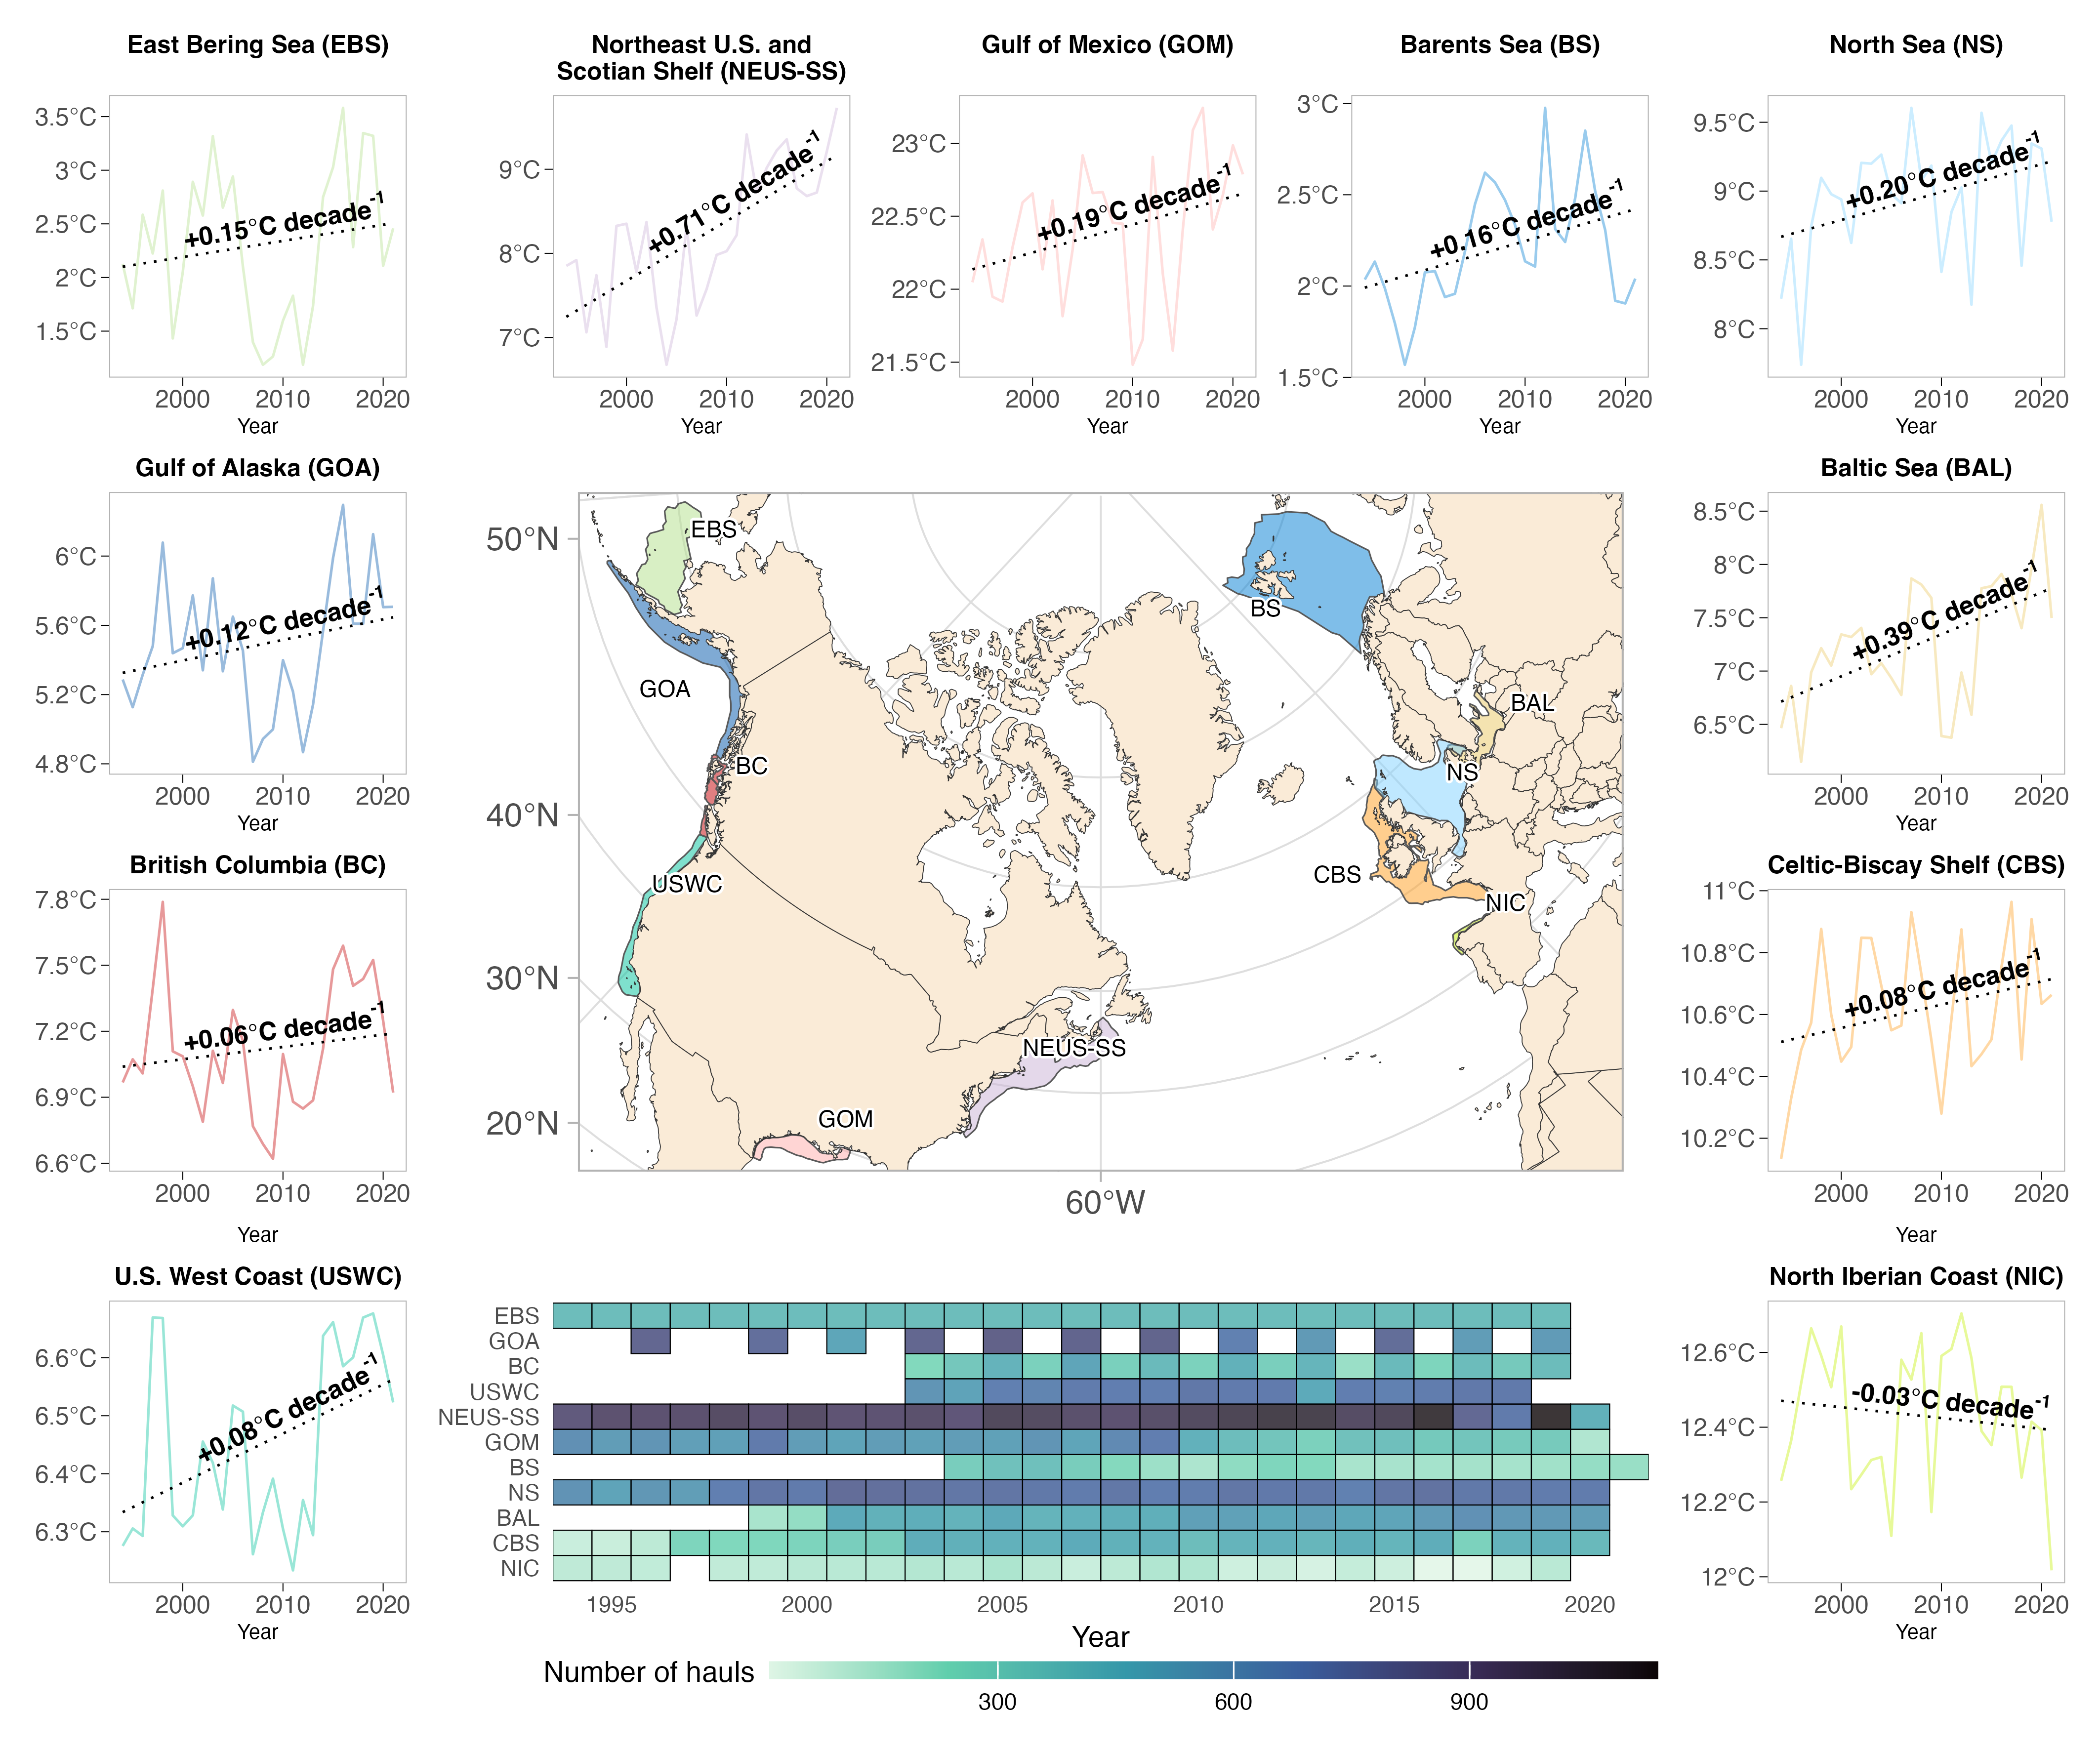
\includegraphics[width=1\textwidth]{output/figures/main/map.png}
\caption{Overview of survey coverage and bottom temperature trends.
The central map shows the regions included in the analysis, with colored polygons indicating survey extents. The tile plot summarizes the number of hauls per region by year. Surrounding panels display regional trends in mean bottom temperature over time; bold values indicate the estimated decadal rate of temperature change.}\label{fig:map}
\end{figure}

\textbf{Prediction grid and environmental matching.} 
After model fitting and validation we predicted species-specific densities on a 4 × 4 km spatial
grid (in local UTM coordinates) covering each region for all years with available data. For each grid cell, we assigned bathymetry and the average bottom temperature over the 12 months preceding the earliest survey month in a region. This procedure generated a consistent spatiotemporal dataset of predicted biomass, depth, and temperature for downstream analyses.

\textbf{Derivation of multi-dimensional distributional metrics and abundance.} To assess species responses to ocean warming, we computed annual metrics that characterize both spatial redistribution and thermal exposure, specifically range centroids (UTM northing and easting), realized depth niche, and realized thermal niche. Horizontal shifts in distribution were quantified using range centroids rather than range edges, as centroids are less susceptible to noise and provide a clearer signal of overall distributional movement, thus offering a more stable and representative measure of geographic displacement \citep{shoo_detecting_2006}. Range centroids were calculated as the biomass-weighted mean UTM northing and easting (center of gravity) across grid cells. The realized depth and thermal niches were computed as biomass-weighted averages of depth and bottom temperature, respectively, summarizing the environmental conditions most intensely occupied by each species (Table~\ref{table:derived_quantities}). All these metrics were derived from biomass density predictions across the spatial grid generated by the fitted spatiotemporal models.

To estimate the annual abundance of each fish population, we calculated an area-weighted relative abundance index by multiplying predicted biomass density by grid cell area, summing these values across all grid cells, and applying a standard bias correction \citep{thorson_geostatistical_2015, thorsonImplementingGeneric2016}.

\textbf{Comparing realized shifts with thermal envelopes shifts.}
To estimate population-specific shifts under climate-driven thermal change, we fitted species distribution models using temperature predictors. These models followed the structure described in \textit{\nameref{sec:Species spatiotemporal modeling}}, but excluded spatiotemporal random fields to focus on direct temperature effects. As predictors, we used (i) the average bottom temperature over the 12 months preceding the earliest survey month in a region, and (ii) the maximum bottom temperature of the previous year. The latter was included to reflect the hypothesis that temperature extremes, rather than means, are more likely to limit species’ ranges \citep{sunday_thermal_2019}. We then derived spatial metrics (range centroid and depth niche) as in \textit{\nameref{sec:Derivation of multi-dimensional distributional metrics and abundance.}}.These temperature-only models provide climate envelope-based expectations under thermal forcing.

\subsection{Bayesian trend analysis}\label{sec:Bayesian trend analysis}

We estimated trends in the set of spatial and thermal metrics described above using multivariate Bayesian mixed-effects models because these metrics are often correlated. For example, depth shifts can co-occur with changes in range centroid, and we modeled them jointly to capture shared variation. We initially modelled the outcomes using a multivariate normal (MVN) distribution, but posterior predictive checks revealed heavier tails than the MVN could capture, so we refitted the model using univariate Student-t distribution for each response, which are more robust to extreme values \citep[e.g.,][]{anderson_black-swan_2017}. Residual correlations across responses were retained using a multivariate normal correlation structure. This change improved predictive accuracy, as confirmed by higher leave-one-out cross-validation (LOO) scores \citep{vehtari_practical_2017} (Supplementary Table~\ref{tab:elpd}).

Next, we compared two alternative random-effects structures using LOO cross-validation: (i) random slopes varying by species–region combinations, and (ii) a hierarchicalstructure with species nested within regions. The nested specification was better supported and was therefore adopted for all subsequent analyses (Supplementary Table~\ref{tab:elpd}). This hierarchical framework improved model fit and, importantly, allowed us to estimate global, regional, and species-level trends within a single unified model.

An alternative would have been to fit separate models for each species and outcome. But this ignores information shared across taxa, regions, and outcomes. Instead, a hierarchical specification applies partial pooling: estimates draw strength from the broader dataset while still allowing region- and species-specific deviations. This shrinkage produces estimates that are more stable than those from independent fits (Supplementary Fig.~\ref{fig:shrinkage}; \citealt{mcelreath_statistical_2018}).


To improve interpretability and aid in model convergence, we mean-centered both the response variables and the time predictor within each species–region combination so that their mean is zero. As a result, the intercept can be omitted. We then rescaled time to decades, so that the slope can be interpreted directly as the rate of change per decade.
Thus the model can be written as:

\begin{align}
y_{i}^{(j)} &\sim \operatorname{Student-t}\left(\nu^{(j)}, \mu_{i}^{(j)}, \sigma^{(j)}\right),\qquad j=1,\dots,4,\\
\mu_{i}^{(j)} &= \beta^{(j)} \cdot \text{decade}_{i} + \beta_{\text{region}[r[i]]}^{(j)} \cdot \text{decade}_{i} + \beta_{\text{species}[s[i]]}^{(j)} \cdot \text{decade}_{i},\label{eq:linearpred} \\
\boldsymbol{\Sigma} &=
\begin{bmatrix}
\sigma_1^2 & \rho_{12}\sigma_1\sigma_2 & \rho_{13}\sigma_1\sigma_3 & \rho_{14}\sigma_1\sigma_4 \\
\rho_{21}\sigma_2\sigma_1 & \sigma_2^2 & \rho_{23}\sigma_2\sigma_3 & \rho_{24}\sigma_2\sigma_4 \\
\rho_{31}\sigma_3\sigma_1 & \rho_{32}\sigma_3\sigma_2 & \sigma_3^2 & \rho_{34}\sigma_3\sigma_4 \\
\rho_{41}\sigma_4\sigma_1 & \rho_{42}\sigma_4\sigma_2 & \rho_{43}\sigma_4\sigma_3 & \sigma_4^2
\end{bmatrix},\\
% OR
\begin{bmatrix}
\varepsilon_i^{(1)} \\ \varepsilon_i^{(2)} \\ \varepsilon_i^{(3)} \\ \varepsilon_i^{(4)}
\end{bmatrix}
&\sim \operatorname{MVN}\!\left(
\mathbf{0},\ 
\operatorname{diag}(\sigma_1,\sigma_2,\sigma_3,\sigma_4)\;
\mathbf{R}\;
\operatorname{diag}(\sigma_1,\sigma_2,\sigma_3,\sigma_4)
\right).
\end{align}

\vspace{1em}

\noindent Here, $y^{(j)}_i$ denotes the response variable $j$ for observation $i$, where $j$ is the latitudinal centroid,
longitudinal centroid, depth niche or thermal niche (Table \ref{table:derived_quantities}). The linear predictor (Eq \ref{eq:linearpred}) includes a global slope of decade for response $j$, denoted $\beta^{(j)}$, along with a deviation in slope for region $r$, $\beta^{(j)}_{\text{region}[r[i]]}$, and a deviation in slope for species $s$ within region, $\beta^{(j)}_{\text{species}[s[i]]}$. Finally,
$\boldsymbol{\Sigma}$ represents the residual covariance matrix capturing residual correlations among the response variables. The scale parameters $\sigma^{(j)}$ are estimated as part of the Student-t and the residual correlation matrix $\mathbf{R}$ controls how residuals co-vary across responses.

We used weakly informative priors for the global slopes (decade effects), guided by published rates of range shifts, depth changes, and ocean warming. For latitudinal and longitudinal centroids, we specified Normal$(0, 50)$ km decade$^{-1}$ priors, which accommodate range shifts up to ~30 km decade$^{-1}$ observed in marine taxa \citep{poloczanska_global_2013}. For depth, we used a Normal$(0, 5)$ m decade$^{-1}$ prior, consistent with estimates of ~3.6 m decade$^{-1}$ deepening in North Sea demersal fish \citep{dulvy_climate_2008}. For thermal niches, we applied a Normal$(0, 0.5)$ °C decade$^{-1}$ prior, encompassing values comparable to the ~0.37 $^\circ$C decade$^{-1}$ observed in rapidly warming shelf seas \citep{chen_longterm_2020}.
For group-level variation in slopes (the standard deviation of year effects), we used $\operatorname{Student-t}$ distributions truncated to $(0,\infty)$ with 3 degrees of freedom, allowing a wide range of biologically plausible variation. Priors were $\operatorname{Student-t}(3, 0, 30)$ km decade$^{-1}$ for spatial centroids, $\operatorname{Student-t}(3, 0, 10)$ m decade$^{-1}$ for depth, and $\operatorname{Student-t}(3, 0, 0.2)$ $^\circ$C decade$^{-1}$ for thermal niches. For species nested within regions, we specified slightly broader priors: $\operatorname{Student-t}(3, 0, 40)$ km decade$^{-1}$ for spatial centroids, $\operatorname{Student-t}(3, 0, 20)$ m decade$^{-1}$ for depth, and $\operatorname{Student-t}(3, 0, 0.4)$ $^\circ$C decade$^{-1}$ for thermal niches. These priors were validated against empirical distributions from the data to ensure consistency with observed variability (Supplementary Fig.~\ref{fig:priors}).

We fit models in R using the \texttt{brms} package \citep{burkner_brms_2017}, which interfaces with Stan via \texttt{rstan} \citep{stan2024,stan_development_team_rstan_2024}. All other priors followed \texttt{brms} defaults. Each model ran with four Markov chain Monte Carlo (MCMC) chains of 4,000 iterations, discarding the first 2,000 as warm-up. The remaining 2,000 samples per chain (8,000 total post–warm-up draws) formed the posterior distribution. Convergence was confirmed by $\hat{R} < 1.01$, absence of divergent transitions, and effective sample sizes $>$ 400 for all key parameters \citep{vehtari_rank-normalization_2021}.

\section{Discussion}\label{sec12}

Discussions should be brief and focused. In some disciplines use of Discussion or `Conclusion' is interchangeable. It is not mandatory to use both. Some journals prefer a section `Results and Discussion' followed by a section `Conclusion'. Please refer to Journal-level guidance for any specific requirements. 

\section{Conclusion}\label{sec13}

Conclusions may be used to restate your hypothesis or research question, restate your major findings, explain the relevance and the added value of your work, highlight any limitations of your study, describe future directions for research and recommendations. 

In some disciplines use of Discussion or 'Conclusion' is interchangeable. It is not mandatory to use both. Please refer to Journal-level guidance for any specific requirements. 

\backmatter

\bmhead{Supplementary information}

If your article has accompanying supplementary file/s please state so here. 

Authors reporting data from electrophoretic gels and blots should supply the full unprocessed scans for key as part of their Supplementary information. This may be requested by the editorial team/s if it is missing.

Please refer to Journal-level guidance for any specific requirements.

\bmhead{Acknowledgements}


\begin{appendices}

\section{Supplementary figures}\label{Appendix A}

\begin{figure}[h]
\centering
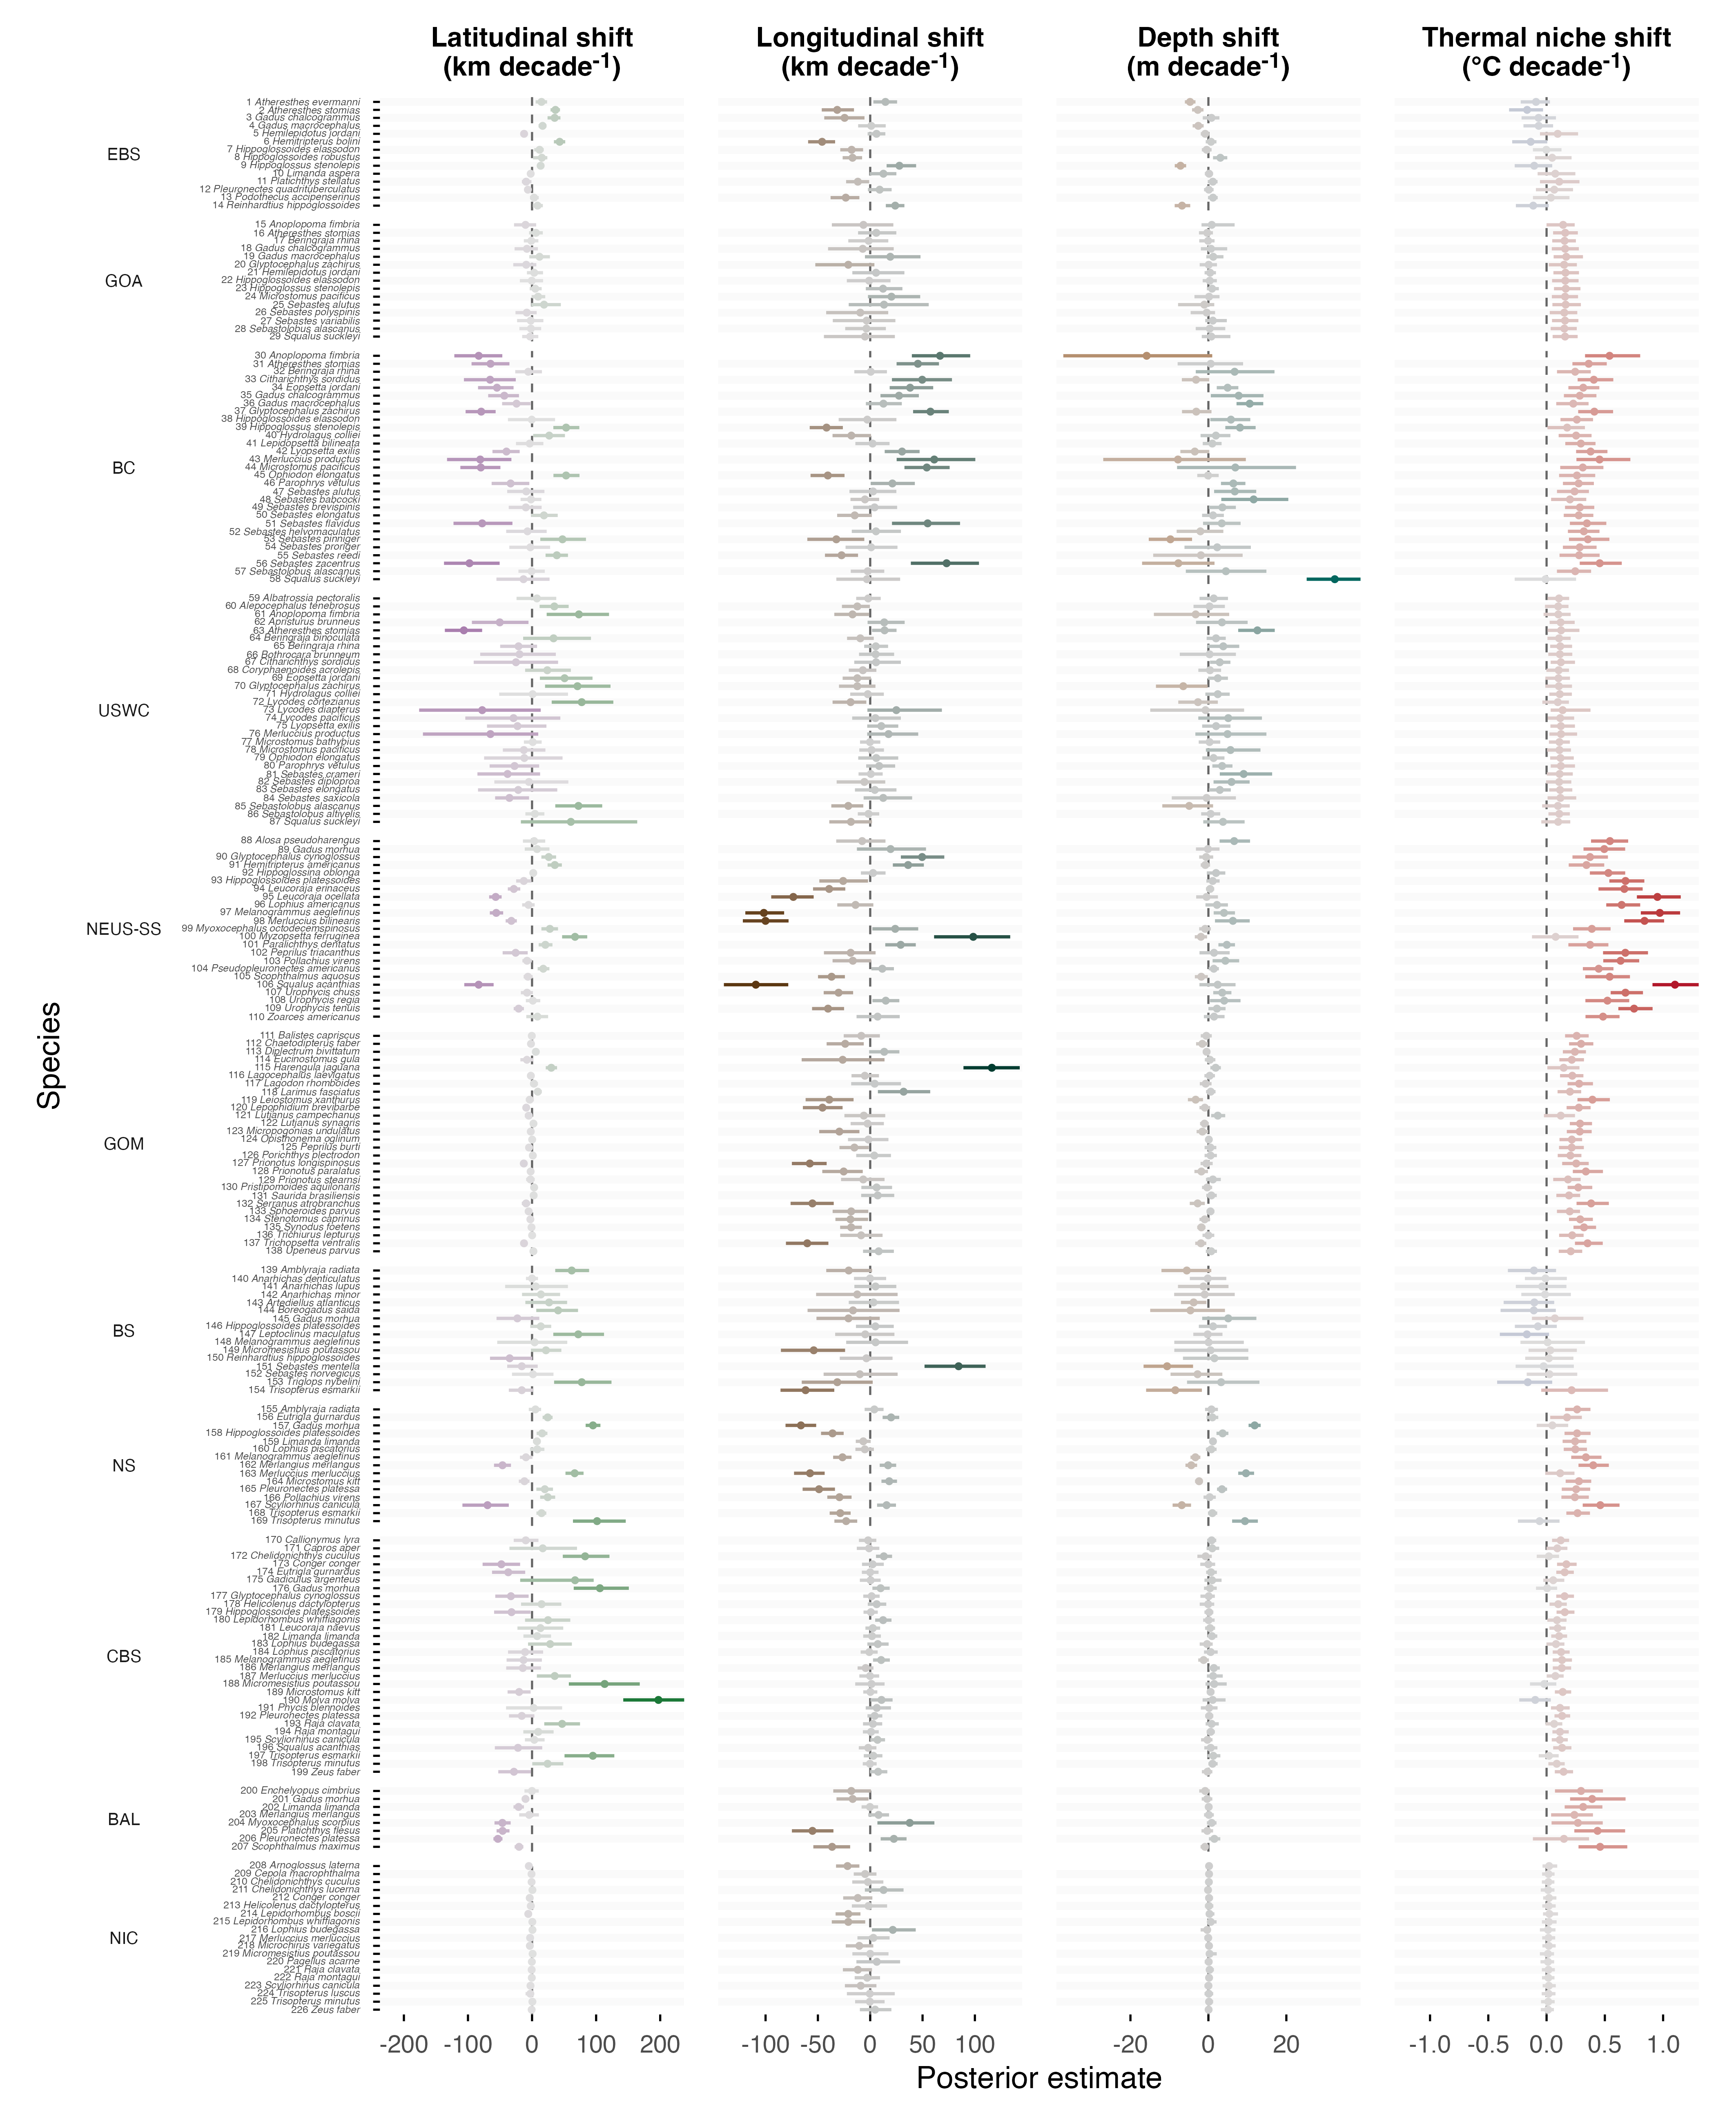
\includegraphics[width=1\textwidth]{output/figures/supp/posterior_slopes_supp.png}
\caption{This is a widefig. This is an example of long caption this is an example of long caption  this is an example of long caption this is an example of long caption}\label{fig:posterior_slopes_supp}
\end{figure}

\begin{figure}[h]
\centering
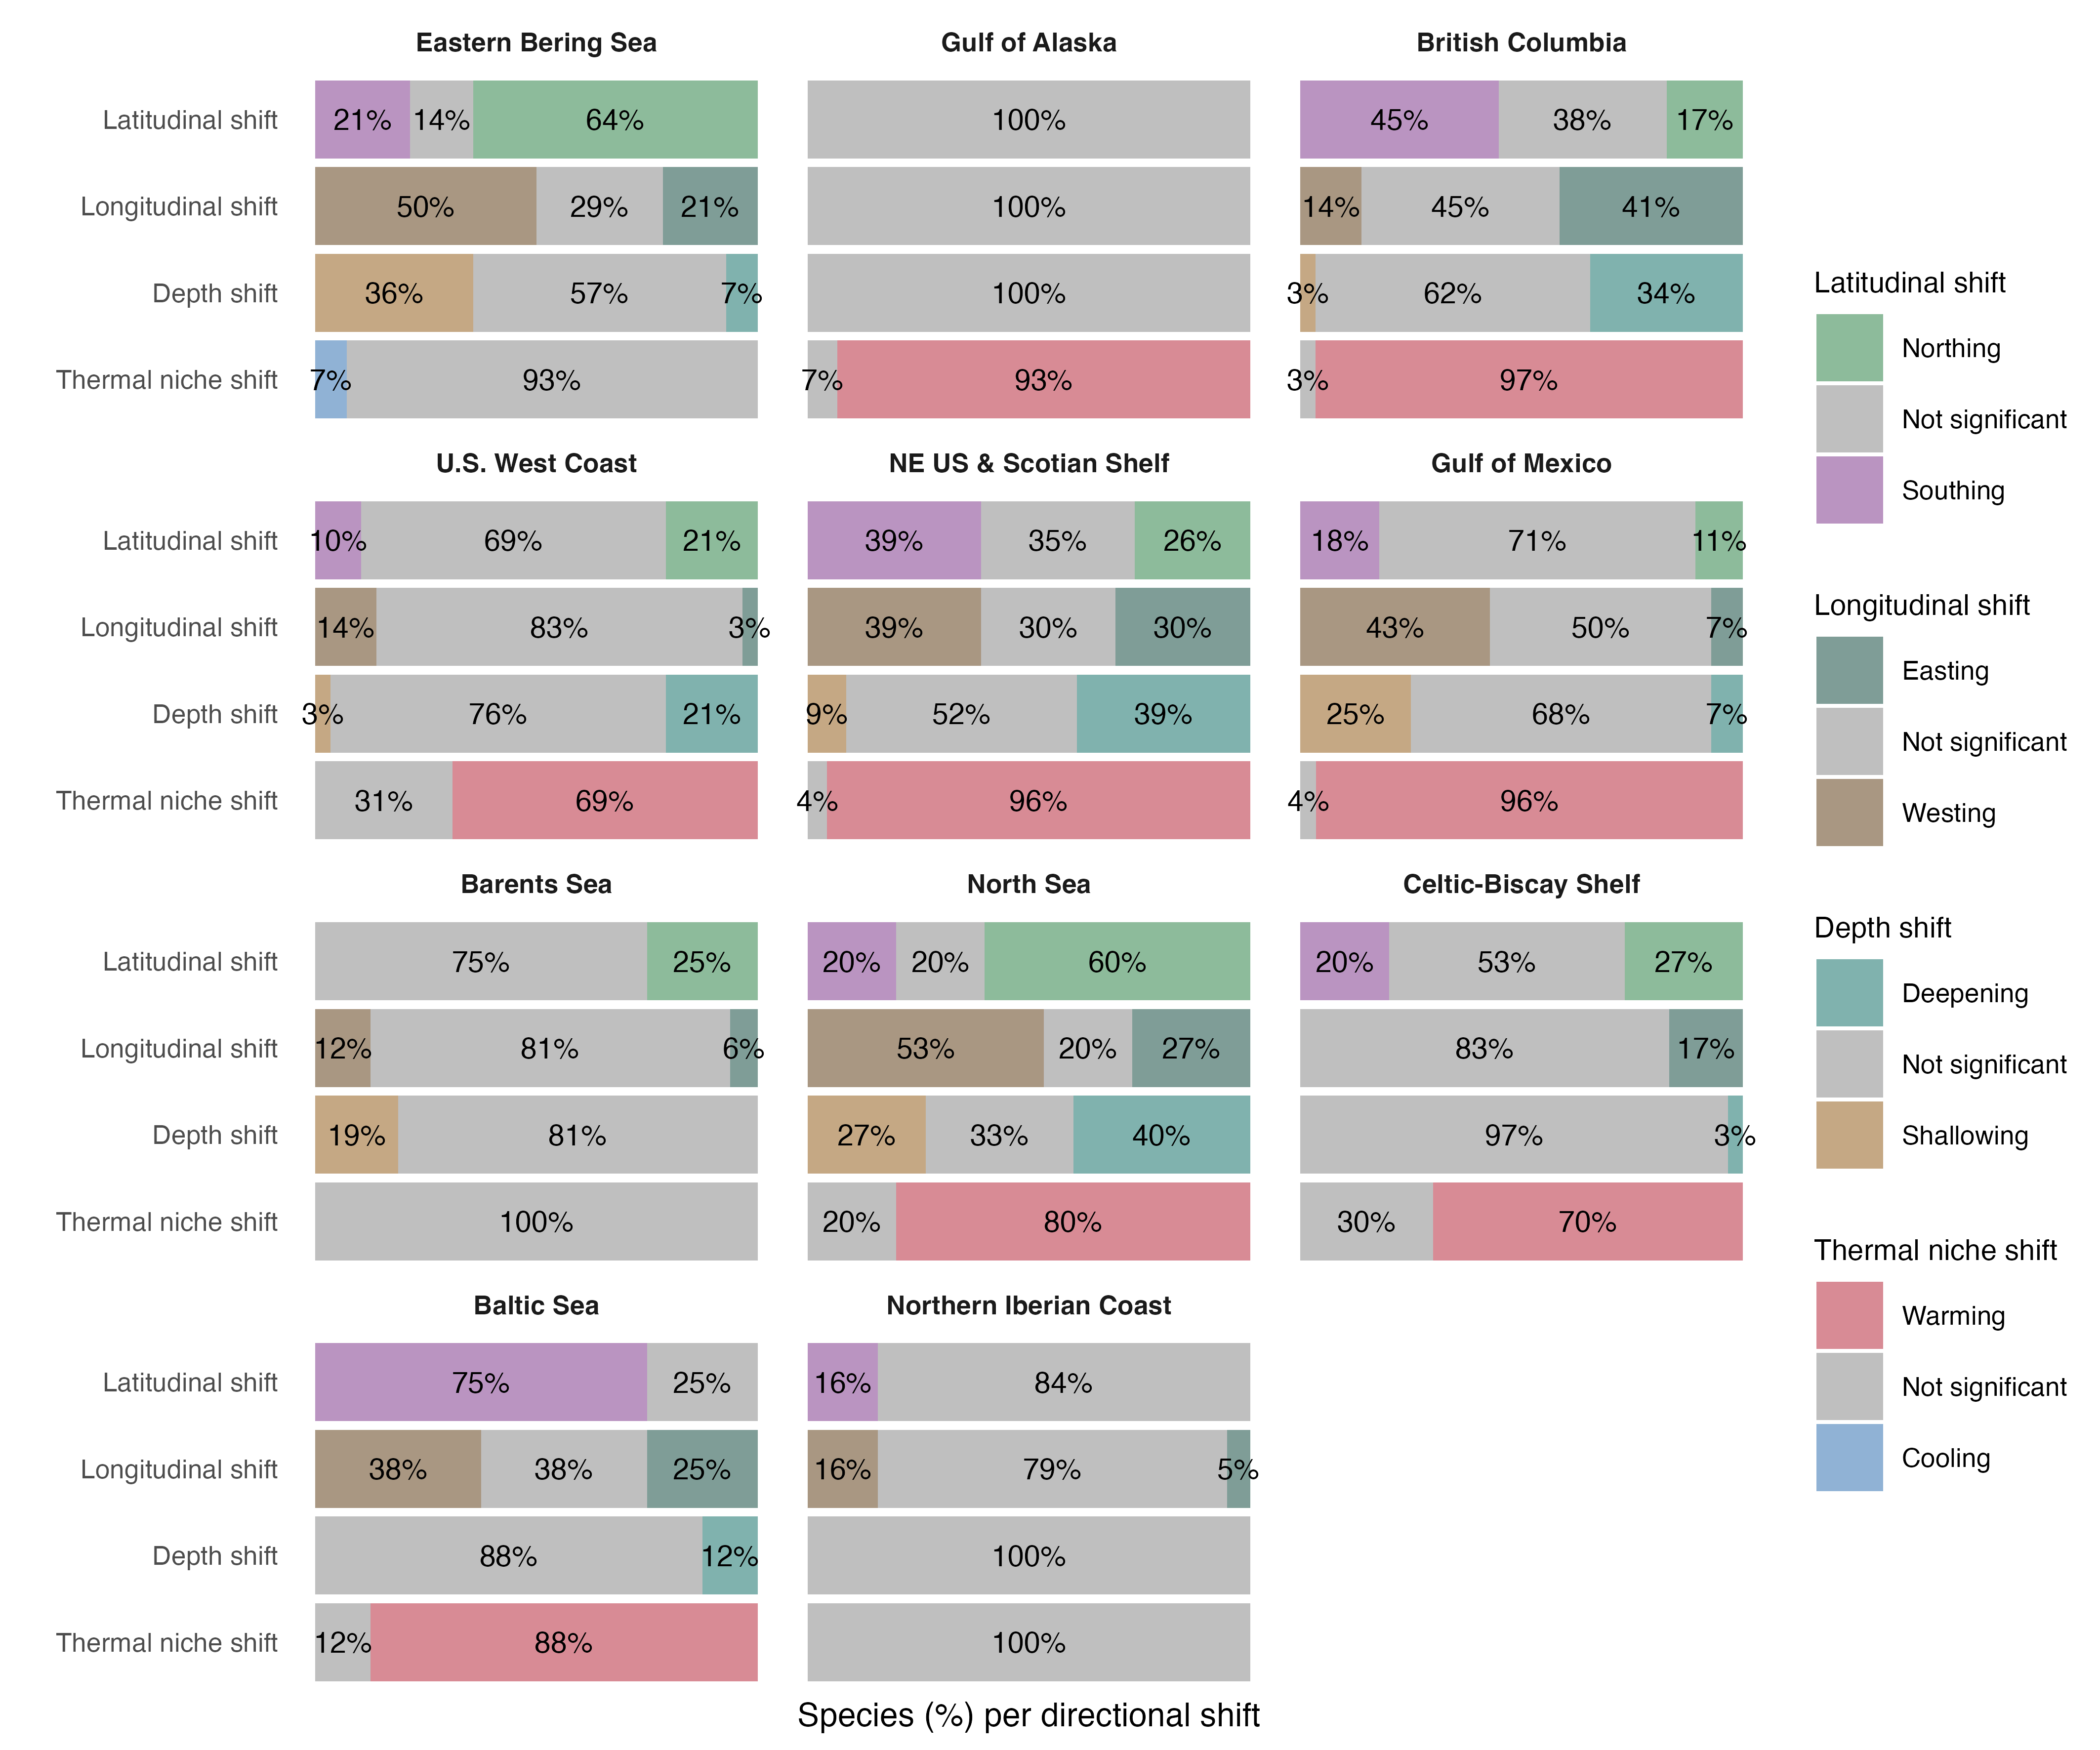
\includegraphics[width=1\textwidth]{output/figures/supp/prop_significant_supp.png}
\caption{This is a widefig. This is an example of long caption this is an example of long caption  this is an example of long caption this is an example of long caption}\label{fig:prop_significant_supp}
\end{figure}

\begin{figure}[h]
\centering
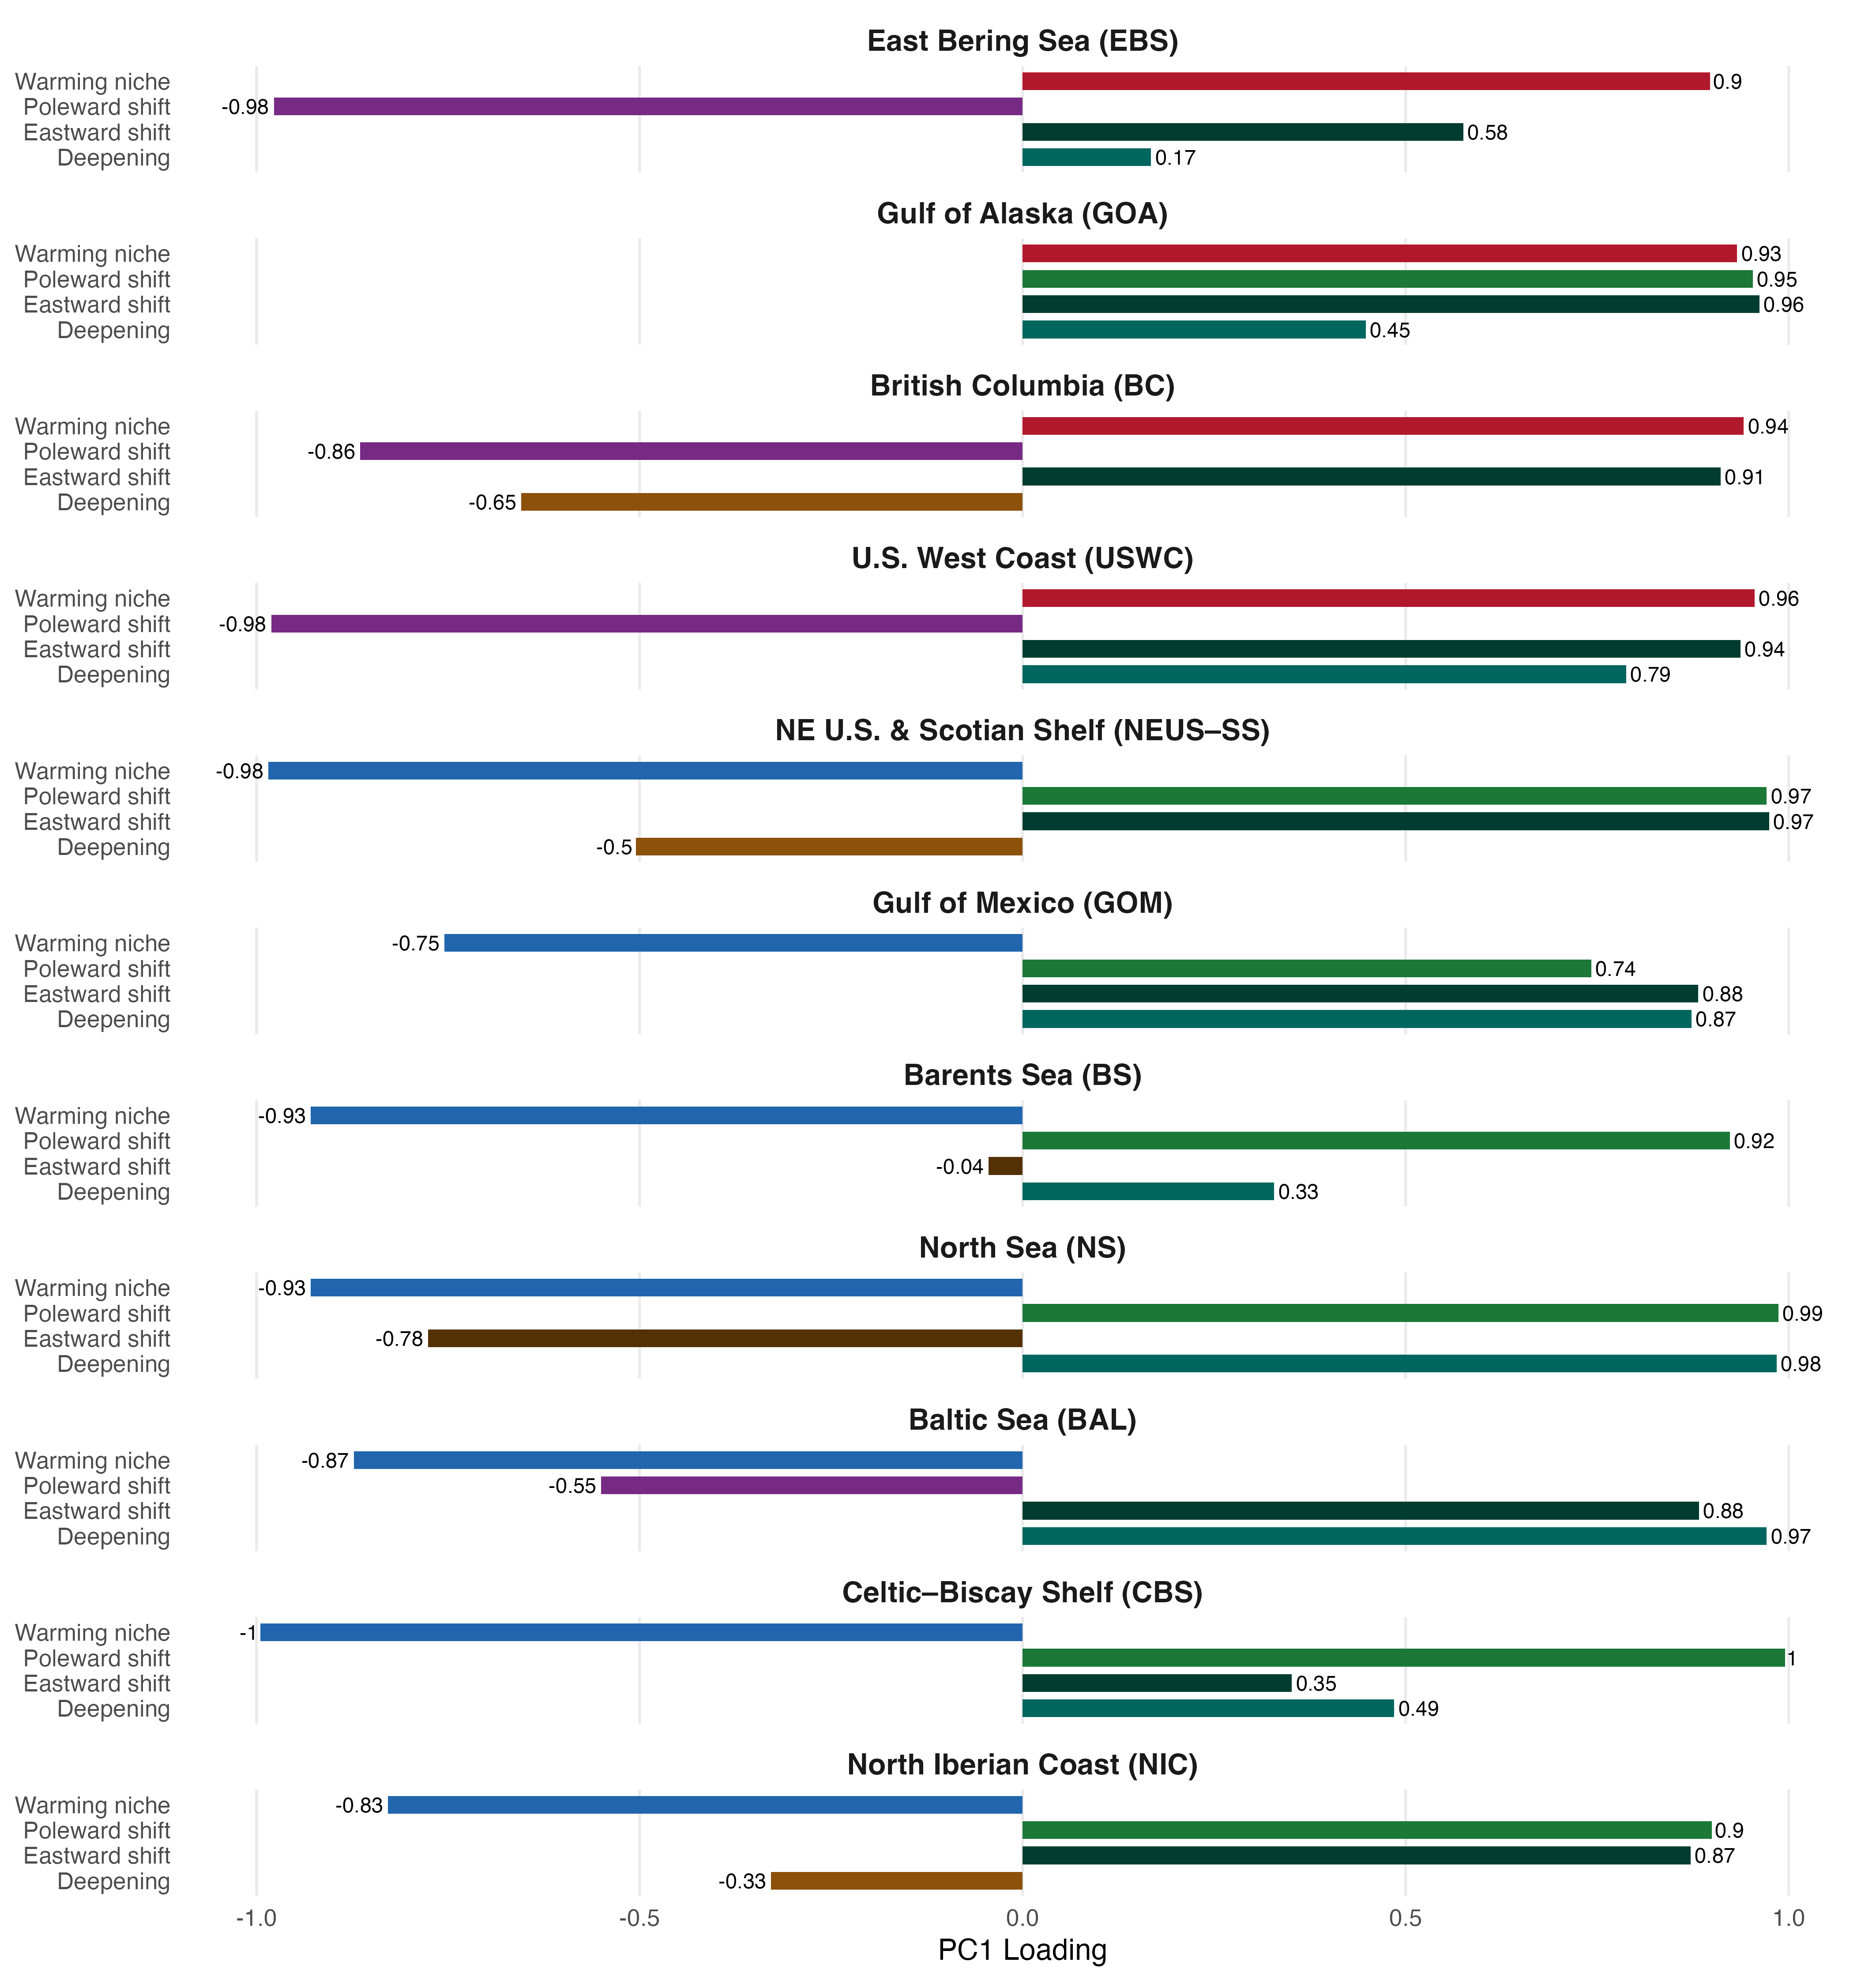
\includegraphics[width=1\textwidth]{output/figures/supp/pca_loadings_supp.png}
\caption{This is a widefig. This is an example of long caption this is an example of long caption  this is an example of long caption this is an example of long caption}\label{fig:pca_loadings_supp}
\end{figure}

\begin{figure}[h]
\centering
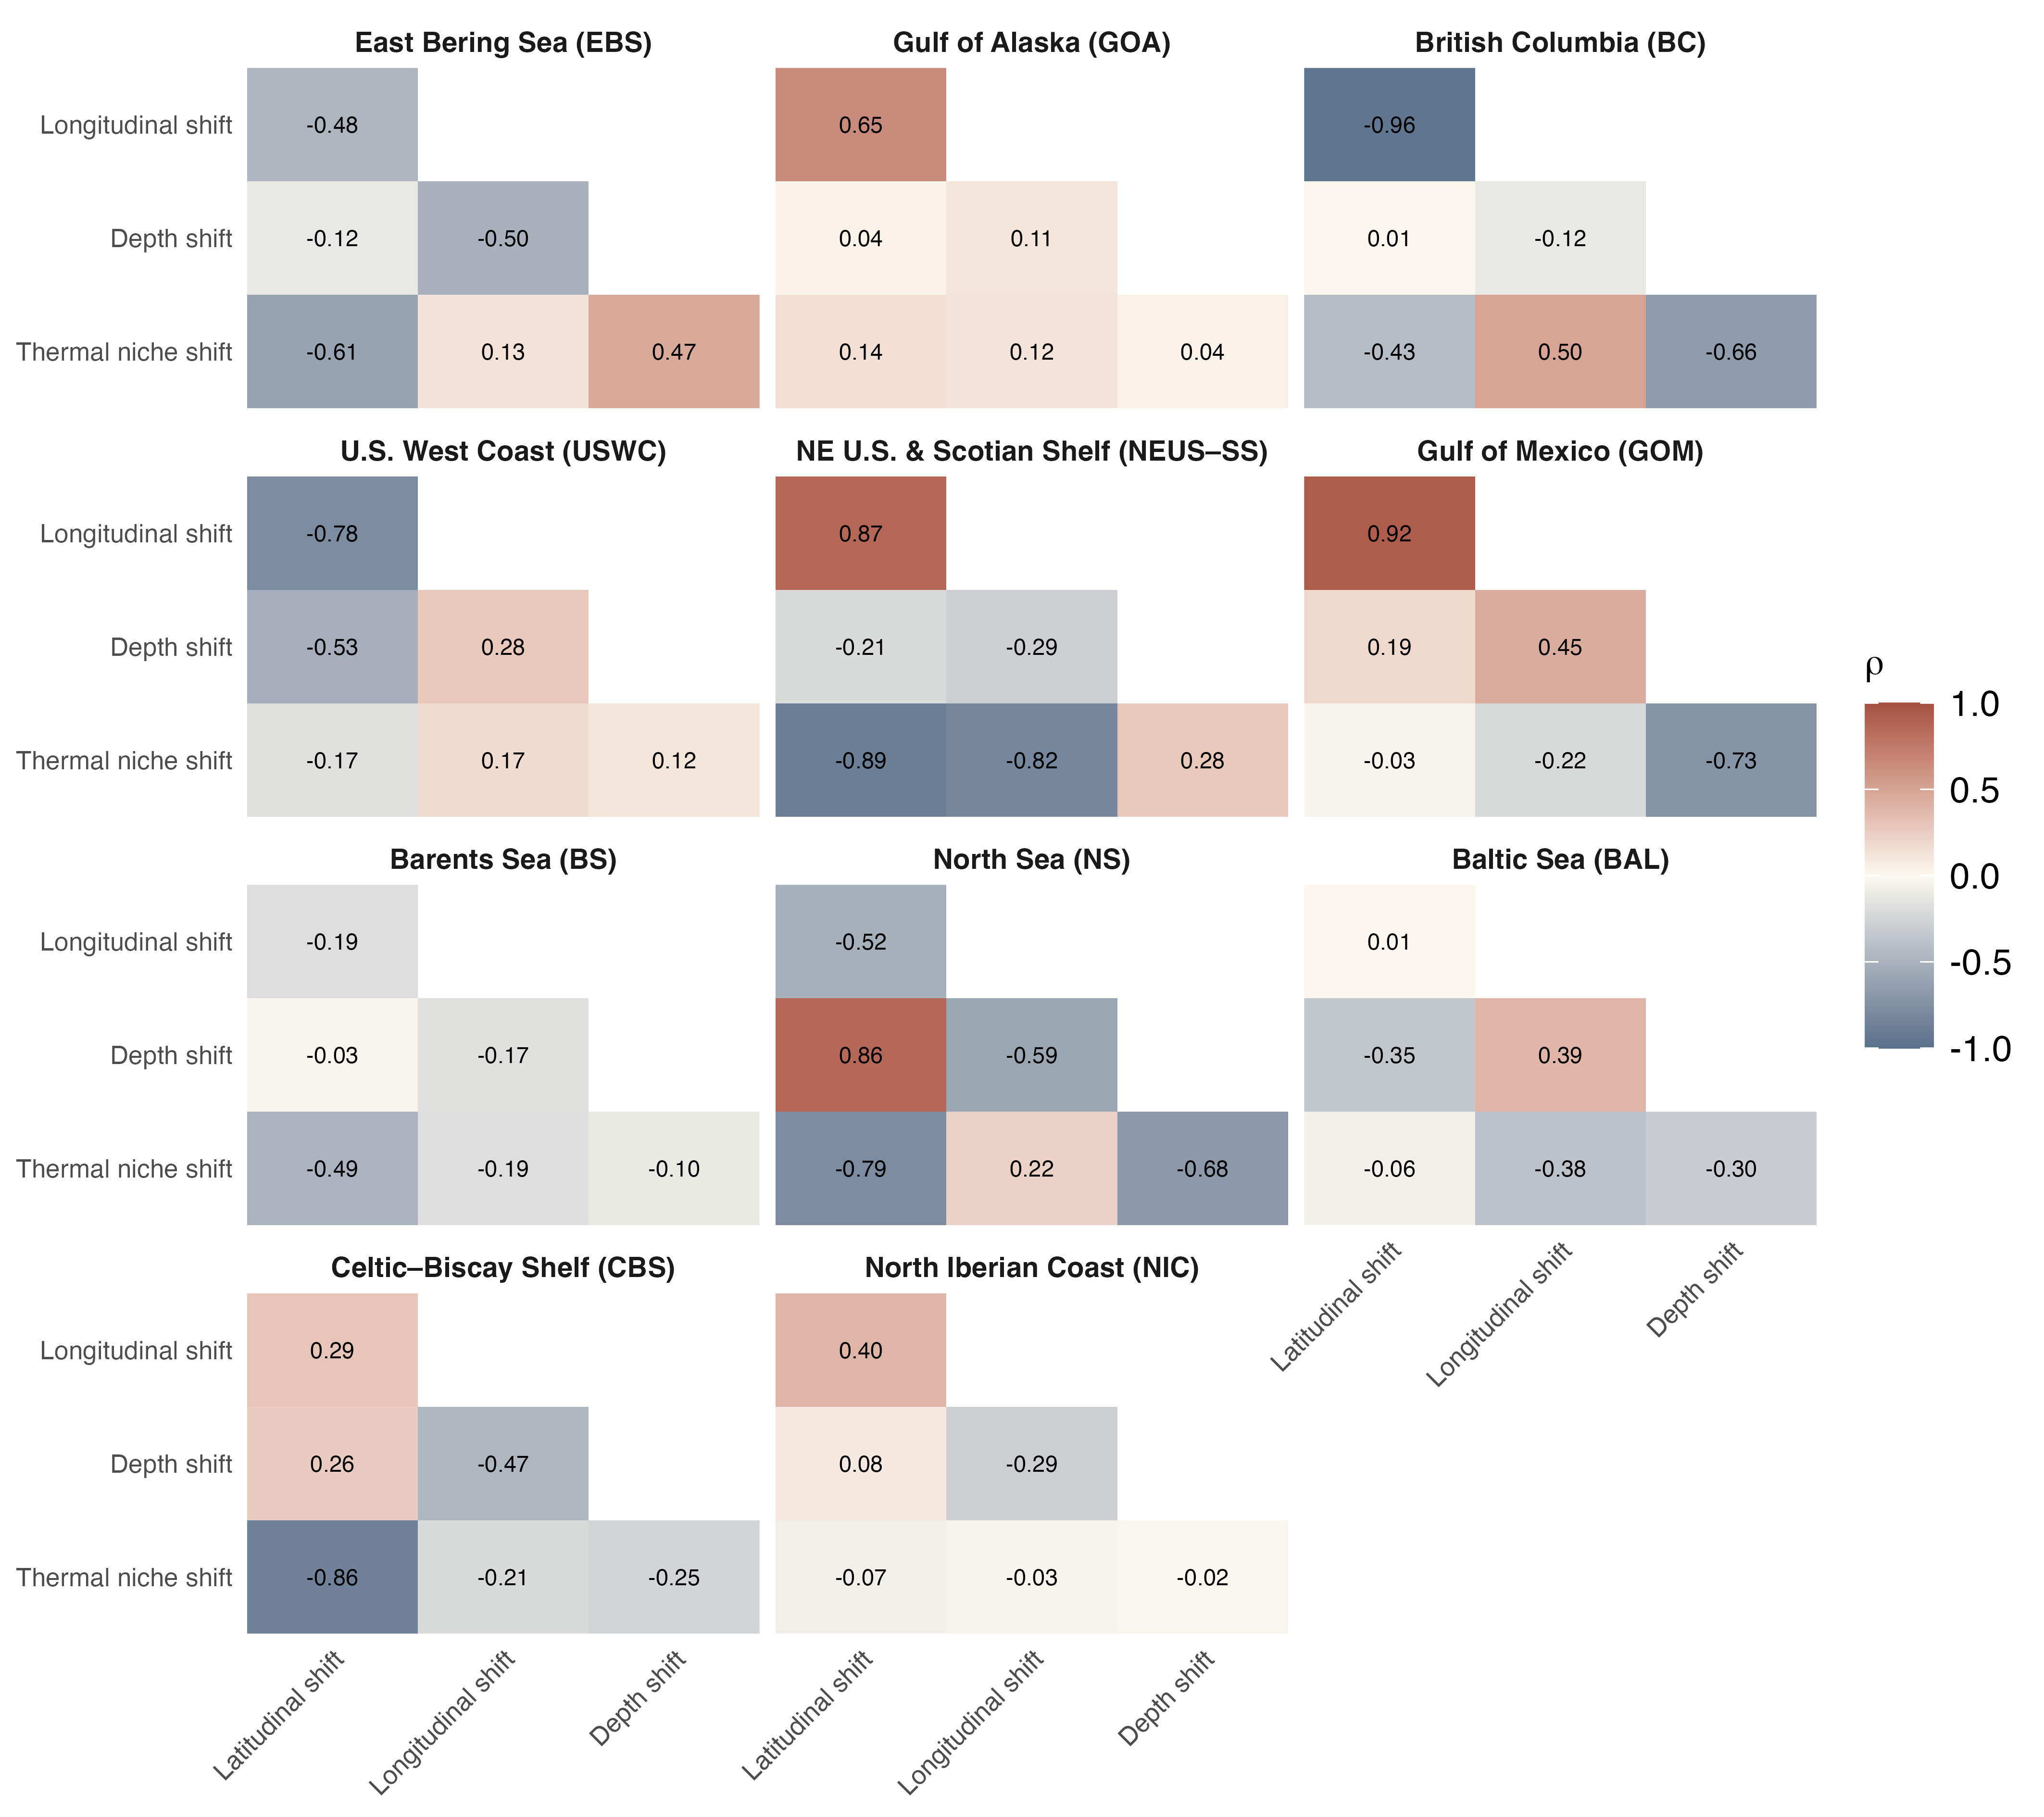
\includegraphics[width=1\textwidth]{output/figures/supp/corr_supp.png}
\caption{This is a widefig. This is an example of long caption this is an example of long caption  this is an example of long caption this is an example of long caption}\label{fig:corr_supp}
\end{figure}

\section{Additional information on spatiotemporal models}\label{Appendix B}
    
The general form of the spatiotemporal GLMM can be represented as:
\begin{align}
    y_{s,t} &\sim \text{Tweedie} \left( \mu_{\boldsymbol{s},t}, p, \phi \right), \quad 1 < p < 2, \label{eq:1} \\
    \mu_{s,t} &= \exp \left( X_{\boldsymbol{s},t} \beta + \omega_{\boldsymbol{s}} + \epsilon_{\boldsymbol{s},t} \right), \label{eq:2} \\
    \omega &\sim \operatorname{MVN} \left(0, \Sigma_{\omega} \right), \label{eq:3} \\
    \epsilon_{t} &\sim \operatorname{MVN} \left(0, \Sigma_{\epsilon} \right), \label{eq:4}
\end{align}
where \( y_{\mathbf{s},t} \) represents fish density (kg/km\(^2\)) at spatial location \( \mathbf{s} \) and time \( t \), \( \mu \) is the expected mean CPUE, and \( p \) and \( \phi \) are the power and dispersion parameters of the Tweedie distribution, respectively. \( \mathbf{X}_{\mathbf{s},t} \) is the design matrix of covariates including year (as a categorical variable) and a second-degree polynomial of log(depth), consisting of both linear and quadratic terms. The vector \( \bm{\beta} \) contains the corresponding fixed-effect coefficients.
We included log-transformed depth as a second-order polynomial to help constrain predictions to plausible magnitudes across the depth gradient.

Because fish species are not constrained by survey boundaries, and some surveys cover only a small part of the distribution range of species we aggregated multiple surveys into broader regions for modeling when appropriate. Surveys with extensive and clearly defined coverage (e.g., the North Sea IBTS) were modeled independently, while those with contiguous spatial domains and partial overlap in time and space (e.g., surveys conducted in British Columbia) were combined (Fig \ref{fig:map}). When multiple surveys were present within a region, we included survey identity as a fixed effect to account for potential differences in sampling. To capture intra-annual variability, we also included a month-specific random intercept for surveys spanning more than three months: $\alpha_m \sim \mathcal{N}(0, \sigma_{\alpha_m}^{2})$, where \textit{m} indexes the sampled months.

The parameters \( \omega_{\mathbf{s}} \) and \( \epsilon_{\mathbf{s},t} \) (Equations \ref{eq:3}--\ref{eq:4}) represent spatial and spatiotemporal random effects, respectively, both modeled as Gaussian Markov random fields \citep{lindgren_explicit_2011}. The spatial random field is shared across years, and represents static spatial effects such as habitat that are not accounted for by the fixed effects, while the spatiotemporal fields represent interannual spatial variation. We assumed spatiotemporal random fields to be independent across years to capture annual variation in spatial structure. While a first-order autoregressive (AR1) process could have been used to model temporal dependence, we opted for the independent formulation to strike a balance between computational efficiency and model flexibility. This approach allows spatial patterns to vary freely from year to year, accommodating potential non-stationary dynamics in species distributions without imposing strict temporal correlation structures.

For British Columbia surveys, which have a biennial sampling structure, we modeled spatiotemporal variation as a random walk process. This modifies Equation \ref{eq:4} into $\epsilon_{\boldsymbol{s},t} \sim  \operatorname{MVN}(\epsilon_{t-1},\Sigma_{\epsilon})$ to allow for flexibility in estimating the spatial and temporal processes in years without data \citep{ward_win_2024}.

Latent spatial and spatiotemporal random fields were approximated using a triangulated mesh with a minimum spacing (cutoff) of 20 km constructed with the \texttt{fmesher} R package \citep{lindgren_fmesher_2025}. This cutoff distance represents the smallest allowed distance between two mesh vertices. We assumed a shared range parameter between the spatial and spatiotemporal fields, while allowing each field to have its own variance.

The maximum marginal log-likelihood was estimated using Template Model Builder \citep[TMB;][]{kristensen_tmb_2016}, which applies the Laplace approximation to integrate out random effects. Models were fit in R 4.1.0 \citep{r_core_team_r_2021} using the \texttt{sdmTMB} package \citep{anderson_sdmtmb_2024}, which interfaces TMB with INLA-based spatial methods \citep{rue_approximate_2009}. Only models with a positive-definite Hessian and a maximum absolute log-likelihood gradient $< 0.001$ were considered successfully converged and used for inference \citep{anderson_sdmtmb_2024}


\section{Additional information on Bayesian trend analysis}\label{Appendix C}

Priors are reported in \ref{tab:priors}

\begin{table}

\caption{\label{tab:priors}Prior distributions for model parameters. Fixed effects ($\beta$), group-level and residual standard deviations ($\sigma$), degrees of freedom ($\nu$) for the Student-t distribution, and the correlation matrix of group-level effects parameterized via its Cholesky factor ($L$). The source column indicates whether the prior was changed from the default.}
\centering
\begin{tabular}[t]{llllll}
\toprule
Prior & Parameter & Coefficient & Group & Response & Source\\
\midrule
LKJ(1) & $\mathbf{L}$ &  &  &  & default\\
Normal(0, 50) & $\beta$ & decade &  & lat centroid & user\\
Normal(0, 50) & $\beta$ & decade &  & lon centroid & user\\
Normal(0, 5) & $\beta$ & decade &  & depth niche & user\\
Normal(0, 0.5) & $\beta$ & decade &  & thermal niche & user\\
\addlinespace
Gamma(2, 0.1) & $\nu$ &  &  & lat centroid & default\\
Gamma(2, 0.1) & $\nu$ &  &  & lon centroid & default\\
Gamma(2, 0.1) & $\nu$ &  &  & depth niche & default\\
Gamma(2, 0.1) & $\nu$ &  &  & thermal niche & default\\
Student-t(3, 0, 30.8) & $\sigma$ &  &  & lat centroid & default\\
\addlinespace
Student-t(3, 0, 28.3) & $\sigma$ &  &  & lon centroid & default\\
Student-t(3, 0, 3.9) & $\sigma$ &  &  & depth niche & default\\
Student-t(3, 0, 2.5) & $\sigma$ &  &  & thermal niche & default\\
Student-t(3, 0, 30) & $\sigma$ & decade & region & lat centroid & user\\
Student-t(3, 0, 30) & $\sigma$ & decade & region & lon centroid & user\\
\addlinespace
Student-t(3, 0, 10) & $\sigma$ & decade & region & depth niche & user\\
Student-t(3, 0, 0.2) & $\sigma$ & decade & region & thermal niche & user\\
Student-t(3, 0, 40) & $\sigma$ & decade & region:species & lat centroid & user\\
Student-t(3, 0, 40) & $\sigma$ & decade & region:species & lon centroid & user\\
Student-t(3, 0, 20) & $\sigma$ & decade & region:species & depth niche & user\\
\addlinespace
Student-t(3, 0, 0.4) & $\sigma$ & decade & region:species & thermal niche & user\\
Student-t(3, 0, 30.8) & $\sigma$ &  &  & lat centroid & default\\
Student-t(3, 0, 28.3) & $\sigma$ &  &  & lon centroid & default\\
Student-t(3, 0, 3.9) & $\sigma$ &  &  & depth niche & default\\
Student-t(3, 0, 2.5) & $\sigma$ &  &  & thermal niche & default\\
\bottomrule
\end{tabular}
\end{table}


%%=============================================%%
%% For submissions to Nature Portfolio Journals %%
%% please use the heading ``Extended Data''.   %%
%%=============================================%%

%%=============================================================%%
%% Sample for another appendix section			       %%
%%=============================================================%%

%% \section{Example of another appendix section}\label{secA2}%
%% Appendices may be used for helpful, supporting or essential material that would otherwise 
%% clutter, break up or be distracting to the text. Appendices can consist of sections, figures, 
%% tables and equations etc.

\end{appendices}

%%===========================================================================================%%
%% If you are submitting to one of the Nature Portfolio journals, using the eJP submission   %%
%% system, please include the references within the manuscript file itself. You may do this  %%
%% by copying the reference list from your .bbl file, paste it into the main manuscript .tex %%
%% file, and delete the associated \verb+\bibliography+ commands.                            %%
%%===========================================================================================%%

\bibliography{references}% common bib file
%% if required, the content of .bbl file can be included here once bbl is generated
%%\input sn-article.bbl

\end{document}
